\documentclass[pdftex,english,10pt,b5paper,twoside]{book}
\usepackage[T1]{fontenc} % In case we want special characters
\usepackage[utf8]{inputenc} % We are all writing in UTF-8

\usepackage[numbers]{natbib} % We need to tweak our referencing a bit.
\usepackage{appendix} % Fixes formatting of appendices
\usepackage[printonlyused]{acronym} % Package to handle the acronym list
\usepackage{graphicx} % We *may* use images
\graphicspath{{images/}} % and it is clean to put them in a separate dir
\usepackage{amstext} % To support \text in math mode
\usepackage{amsmath}
\usepackage{hyperref} % Internal and external links is nice
\hypersetup{
    pdfborder=0 0 0, % ..especially without red borders
    pdftitle={Cloud Storage Vault},
    pdfauthor={Haver, Melvold and Ruud},
    pdfsubject={Secure Storage in the Cloud},
    pdfkeywords={NTNU, thesis, secure, cloud, cryptographic, sharing}
}

% Packages and settings for code listings
\usepackage{listings}
\usepackage{caption}
\usepackage{upquote}
\usepackage{xcolor}
\DeclareCaptionFont{white}{\color{white}}
\DeclareCaptionFormat{listing}{\colorbox{gray}{\parbox{\textwidth}{#1#2#3}}}
\captionsetup[lstlisting]{format=listing,labelfont=white,textfont=white}
\lstset{
language=Java,
keywordstyle=\bfseries\ttfamily\color[rgb]{0,0,1},
identifierstyle=\ttfamily,
commentstyle=\color[rgb]{0.133,0.545,0.133},
stringstyle=\ttfamily\color[rgb]{0.627,0.126,0.941},
showstringspaces=false,
basicstyle=\small,
numberstyle=\footnotesize,
numbers=left,
stepnumber=1,
numbersep=10pt,
tabsize=2,
breaklines=true,
prebreak = \raisebox{0ex}[0ex][0ex]{\ensuremath{\hookleftarrow}},
breakatwhitespace=false,
aboveskip={1.5\baselineskip},
columns=fixed,
upquote=true,
extendedchars=true,
frame=bottomline,
inputencoding=utf8
}

% Set equal margins on book style
% \usepackage{layout} % Use \layout to print out the margins (debug)
%\usepackage{geometry}
%\geometry{bindingoffset=1cm}
\usepackage[lmargin=25mm,rmargin=25mm,tmargin=27mm,bmargin=30mm]{geometry}

% Restyle chapter headers
\usepackage{fix-cm}
\makeatletter
\renewcommand{\@makechapterhead}[1]{%
  \vspace*{50\p@}%
  {\parindent \z@ \raggedright \normalfont
    \vspace{15pt}%
    \ifnum \c@secnumdepth >\m@ne
        %\hfill\huge\scshape \@chapapp\space
        \hfill\fontsize{60}{90}\selectfont \thechapter % Chapter number
        \par\nobreak
        \vskip 20\p@
    \fi
    \interlinepenalty\@M
    \hfill \Huge \scshape #1\par % Chapter title
    \vspace{5pt}
    \hrule
    \nobreak
    \vskip 40\p@
  }}
\makeatother

\author{Eirik Haver \and Eivind Melvold \and Pål Ruud}
\title{Master thesis - Cloud Storage Vault}
\date{\today}

\begin{document}

\chapter*{Problem Description}
\thispagestyle{empty}
\pagestyle{empty}

Modern cloud storage systems that encrypts data for "at rest" protection often
has access to the stored data, since the encryption is performed with an
encryption key known by the service provider.\\

\noindent The candidates will design an application in which all data stored in
the cloud are encrypted with a key that cannot be obtained by the service
provider.\\

\noindent Other goals of the application should be the ability to share
encrypted files with others users, without leaking the encryption key to the
service provider, and make it as user friendly as possible without compromising
security. The students will develop a proof of concept implementation of the
design.\\

\medskip\noindent
\begin{tabbing}
    Assignment given: \hspace{12pt} \= 24. January 2011 \\
    Supervisor: \> Danilo Gligoroski\\
    External Supervisors: \> Carsten Maartmann-Moe, Ernst \& Young AS\\
    \> Antonio Martiradonna, Ernst \& Young AS
\end{tabbing}

\chapter*{Abstract}
\addcontentsline{toc}{chapter}{Abstract}
\pagestyle{plain}
\pagenumbering{Roman}
\setcounter{page}{1}

%  Writers should follow a checklist consisting of:
% Motivation: Why do we care about the problem and results?
% Problem Statement: What problem are we trying to solve? Scope/limits.
% Approach: How did we go about solving or making progress on the problem?
% Results: What is the answer? Numbers, not vague 'very', 'small' etc.
% Conclusions: What are the implications of your answer? Further work.
%
%  Each section is typically a single sentence, although there is room for
%  creativity.

Today, major IT-companies, such as Microsoft, Amazon and Google, are offering
online storage services to their customers. This is a favourable solution -- as
opposed to regular storage -- in terms of low costs, reliability, scalability
and capacity. However, important security features such as data privacy and
integrity are often absent.

To address these issues, a cryptographic architecture is proposed, that ensures
the confidentiality and integrity of the data stored by users, independent of
the trust of the underlying provider. It also includes secure sharing of
private data among customers of the same provider. The scheme was further
implemented as a proof of concept.

The underlying cryptographic architecture is based on existing open source
systems and cryptographic primitives. The architecture was further implemented
as a reusable general library in Java. An Android client was created and
several performance tests were conducted\footnote{Source code available at
\url{https://github.com/zerqent/cloud-storage-vault/}}.

The proof of concept system shows that it is possible to implement the proposed
scheme and that the cryptographic operations does not significantly affect the
user experience on an Android device. Weaknesses of the scheme are identified.

We present a scheme for secure storage and sharing of files on an untrusted
server, and argue for its validity. To support streaming functionality, the
scheme could be extended with hash trees to validate small parts of a file at
the time.

\chapter*{Preface}
\addcontentsline{toc}{chapter}{Preface}

The work behind this report was carried out during the spring semester in 2011
at the Norwegian University of Science and Technology (NTNU), Institute of
Telematics (ITEM). The report is the final result of a master thesis in
information security written by three graduate students at NTNU. The thesis was
assigned by Ernst \& Young AS Norway, and acknowledged by ITEM.

\vspace{13pt}

We would like to thank our external supervisors Carsten Maartmann-Moe and
Antonio Martiradonna, at Ernst \& Young AS, for their valuable contributions.
We would also like to thank Danilo Gligoroski at the Department of Telematics
for providing constructive feedback throughout the semester, and for giving us
the opportunity to write this thesis. In addition, we would like to thank all
contributors of code and documentation to the open source software Tahoe-LAFS,
which has given us great inspiration and building blocks for our thesis.

\vspace{13pt}

Best regards,
\begin{center}
Eirik Haver, Eivind Melvold and Pål Ruud
\vspace{13pt}

June, 2011

\end{center}

\tableofcontents

\cleardoublepage
\phantomsection
\addcontentsline{toc}{chapter}{\listfigurename}
\listoffigures

\cleardoublepage
\phantomsection
\addcontentsline{toc}{chapter}{\listtablename}
\listoftables

\cleardoublepage
\phantomsection
\addcontentsline{toc}{chapter}{\lstlistlistingname}
\lstlistoflistings
\cleardoublepage

\chapter*{Acronyms}
\addcontentsline{toc}{chapter}{Acronyms}

\begin{acronym}[PBKDF2]
\acro{ACL}{Access Control List}
\acro{AES}{Advanced Encryption Standard}
\acro{API}{Application Programming Interface}
\acro{BFDA}{Brute Force and Dictionary Attack}
\acro{CA}{Certification Authority}
\acro{CBC}{Cipher Block Chaining}
\acro{CDA}{Cluster Dictionary Attack}
\acro{CSPRNG}{Cryptographically Secure Pseudorandom Number Generator}
\acro{CPU}{Central Processing Unit}
\acro{CSV}{Cloud Storage Vault}
\acro{CTR}{Counter}
\acro{DRY}{Don't Repeat Yourself}
\acro{DSA}{Digital Signature Algorithm}
\acro{DSS}{Digital Signature Scheme}
\acro{EC2}{Elastic Compute Cloud}
\acro{ECB}{Electronic Codebook}
\acro{FAQ}{Frequently Asked Questions}
\acro{GPU}{Graphics Processing Unit}
\acrodef{GUI}{Graphical User Interface}
\acro{FEC}{Forward Error Correction}
\acro{HDFS}{Hadoop Distributed File System}
\acro{HTTP}{Hypertext Transfer Protocol}
\acro{HTTPS}{Hypertext Transfer Protocol Secure}
\acro{IaaS}{Infrastructure as a Service}
\acro{IV}{Initialization Vector}
\acro{JCA}{Java Cryptography Architecture}
\acro{JCE}{Java Cryptographic Extensions}
\acro{JDK}{Java Development Kit}
\acro{JRE}{Java Runtime Environment}
\acro{JVM}{Java Virtual Machine}
\acro{LAFS}{Least Authority File System}
\acro{MAC}{Message Authentication Code}
\acro{MITM}{Man-in-the-middle}
\acro{NIST}{National Institute of Standards and Technology}
\acro{OS}{Operating System}
\acro{P2P}{Peer-to-Peer}
\acro{PBKDF2}{Password-Based Key Derivation Function version 2}
\acro{PaaS}{Platform as a Service}
\acro{PasS}{Privacy as a Service}
\acro{PEP}{Python Enhancement Proposal}
\acro{PGP}{Pretty Good Privacy}
\acro{PKI}{Public Key Infrastructure}
\acro{QR}{Quick Response}
\acro{RAM}{Random Access Memory}
\acro{ROM}{Read Only Memory}
\acro{REST}{Representational State Transfer}
\acro{RSA}{Rivest, Shamir and Adleman}
\acro{SaaS}{Software as a Service}
\acro{SDK}{Software Development Kit}
\acro{SHA}{Secure Hash Algorithm}
\acro{SQL}{Structured Query Language}
\acro{SSL}{Secure Socket Layer}
\acro{TCCP}{Trusted Cloud Computing Platform}
\acro{TCG}{Trusted Computing Group}
\acro{TLS}{Transport Layer Security}
\acro{TPM}{Trusted Platform Module}
\acro{TTP}{Trusted Third Party}
\acrodef{UMTS}{Universal Mobile Telecommunications System}
\acro{URI}{Uniform Resource Indetifier}
\acro{URL}{Uniform Resource Locator}
\acrodef{USB}{Universal Serial Bus}
\acro{VM}{Virtual Machine}
\acro{WPA}{Wi-Fi Protected Access}
\acro{WSGI}{Web Server Gateway Interface}
\end{acronym}

%**************************************%
\chapter{Introduction}
\label{ch:intro}
%**************************************%
\pagenumbering{arabic}
\setcounter{page}{1}

The term \emph{Cloud Computing} is not clearly defined \cite{clouddef}, but
involves the provision of software or computational resources available by
demand via the Internet.  In a draft \cite{cloud_nistdef}, the \ac{NIST}
defines cloud computing as:

\begin{quote}\it ``Cloud computing is a model for enabling ubiquitous,
convenient, on-demand network access to a shared pool of configurable computing
resources (e.g., networks, servers, storage, applications, and services) that
can be rapidly provisioned and released with minimal management effort or
service provider interaction.'' \end{quote}

More and more of the traditionally locally hosted services are moving to the
cloud. The amount of flexibility and cost savings this provides, can be
extensive.

Today, we take the services that the established cloud providers offer us for
granted. For example, both Google and Microsoft provide services for online
document editing, email, file storage and more for free, and available at any
time from anywhere \cite{googleservices, microsoftservices}.

However, this often comes at a cost of reduced privacy, as the control over the
hosting environment is lost. Users are therefore forced to increasingly think
about how the data stored online can leak to unwanted people, either by
accident, or by purpose by unfaithful servants. Should it be sufficient to
trust the security policies of the providers, or is it possible to handle the
privacy issues locally?

This thesis deals with these question and suggests a scheme to make data stored
in the cloud secure. We define the criteria of a secure storage system as
follows.

\begin{enumerate}
  \item Only authorized people can access the data.
  \item Confidentiality is to be assured in a safe environment prior to
  storing data at the provider.
  \item An intrusion of the server does not affect the confidentiality of the
  data.
  \item It is possible to verify the integrity of the stored data.
  \item The storage scheme is documented in detail, such that users can
      easily understand the scheme and accept it on that basis.
  \item An implementation of the storage scheme is open source.
  \item The use of a trusted third party is not mandatory.
\end{enumerate}

\section{Motivation}

%In the last decade, the available supply for services that offer data storage
%remotely in the cloud has increased considerable. Storing private data at a
%third party provider, in contrast to self-hosted storage devices, has proven to
%be preferable due to low storage costs and high reliability, scalability and
%capacity.
%
%However, storing data at a remote location prevents users from physically
%protecting their storage medium. With this in mind, there is no guarantee that
%the data of customers is kept private and secure from unfaithful servants at the
%storage provider.

There has lately been introduced numerous applications and architectures
\cite{tahoe, tccp, PasS} that ensure privacy and integrity of data stored at an
untrusted provider. However, many of these alternative systems are missing one
or more properties towards being, as we define it, a completely secure cloud
storage solution. This has motivated us to create a scheme that solves all of
these challenges.

Additionally, we do see this as a golden opportunity to learn more about
software development, development methodologies, team work, and practical use
of information security and cryptography.

\section{Related Work}

In the later years, there has been a lot of research done in the field of
security in cloud computing. The problems that arise are fundamentally not
different from those revealed by classic information security scenarios. The
key point is that when using a service hosted by someone you do not know, you
have to treat that \emph{someone} as untrusted and as a possible attacker.
Generally speaking, you loose control over the hosting environment, and hence
has to deal with the security issues this implies.

In Section \ref{sec:research}, we present four papers \cite{PasS,
privacymanager, tccp, microsoftresearch} which try to solve security issues in
a shared hosting environment. Common to all of these, is that they either rely
on special, secure and tamper-proof hardware and/or a trusted third party.

Another way of providing a solution to the same problem, is to give the
responsibility of the security operations to the client, i.e. in an environment
that the user has control of. In Section \ref{sec:existing}, we present three
publicly available software services that relates to this approach.

One of these applications, Tahoe-\ac{LAFS} \cite{tahoe}, is given special
attention. This is because it is an open source and a well documented piece of
software, that answers most of the problems arising in an untrusted cloud
storage environment, thus it relates closely to the work performed in this thesis.

\section{Scope and Objectives} 
\label{sec:criteria} 

There are two main objectives for this thesis, the first is to make a
cryptographic scheme that fulfils the criteria mentioned in the introduction.
The scheme shall in addition provide the possibility of sharing stored data
between multiple cloud storage users, while sustaining desired security. The
underlying scheme for sharing data should further be applicable for both
enterprise and personal user scenarios.

The second main objective is to implement the proposed scheme as part of a
proof of concept application for Android devices. The application shall be
designed for personal users and implement the most necessary features, and be
measured in security and performance.

Finally, it is important that the implementation of the cryptographic scheme
should be available as open source and well documented. This criterion exists
because the security should be verifiable to anyone interested in using the
software. In addition, we believe open source encourages participation and
analysis of the system which in turn will lead to a more secure system.

\section{Limitations}

We will focus on making an architecture that covers the scope and objectives,
in an easy to understand and thorough way. In addition, making core
functionality, that demonstrates the most important security features in a proof
of concept system, will be prioritized.

However, due to time and resource constraints, we will focus less on the following:
\begin{itemize}
  \item The language in the proof of concept client should be clear, but the
    \ac{GUI} itself will not be prioritized
  \item Experimentation with the proof of concept code, other
    than basic performance and security measurements
  \item Experimentation with the proof of concept client on hardware equipment
    other than what we easily have available at the time of testing
\end{itemize}

\section{Methodology}
\label{methodology}

The work behind this thesis, is carried out by the three authors in
cooperation. The methodology used, can be categorized based on the three main
parts of this work; the \emph{research}, the \emph{design and abstraction}
part, and the \emph{software development} cycles.

The research will include an analysis of related systems, and a study of
relevant background theory. Based on this theory, we will use experimentation
to create and design a theoretical solution to the problem of secure storage
and sharing of files on an untrusted server. We will work by iteratively
analysing our experimentation to find and correct flaws with the design.

The third part of the work, is the software development cycles of the proof of
concept application.

\paragraph{SCRUM} We will work after SCRUM principles -- an iterative and
incremental based framework for project management \cite{scrum}. There does not
exist a SCRUM \emph{product owner} for the system we will create, nor do we
fulfil the requirements and characteristics of a traditional SCRUM
\emph{team}\cite{scrum}. Hence, we will use the principles that are practically
possible for us to follow:

\begin{itemize}
  \item Daily \emph{stand-up} with planning of the tasks of the current day
  \item Weekly \emph{sprint}\footnote{A \emph{sprint} is a defined period with
    a given set of tasks.} planning meetings
  \item Keep tasks on stickers, that we move between different phases on a
    board: \emph{to do}, \emph{in progress}, \emph{quality assurance} and
    \emph{done}. This is to keep track of progress in the current sprint
  \item Continuously analyse the process, and improve it if possible
\end{itemize}

\paragraph{DRY} We choose to follow the \ac{DRY} principle when developing
software. \citet{dry} define \ac{DRY} as:

\begin{quote}\it
Every piece of knowledge must have a single, unambiguous, authoritative
representation within a system.
\end{quote}

\noindent This principle can be taken further, as to not develop something that
has already been developed in the past. If there exist a library for a given
task that does fulfil the requirements set for the specific task, we will
choose to utilize the library instead of developing similar code by ourselves.

\section{Outline}

This thesis is presented as per the following chapters:

\paragraph{Chapter \ref{ch:background} -- Background} provides background
knowledge of the security services, technologies and software used to form a
secure cloud storage system. In addition, relevant research and commercial
solutions are scrutinized.

\paragraph{Chapter \ref{ch:technical} -- Technical Procedure} goes through the
development process of the scheme and software produced by this thesis. It
starts with an overview of the architectural properties, followed by the more
specific cryptographic scheme that fits in with the architecture. Lastly, the
implementation of the proof of concept system is described.

\paragraph{Chapter \ref{ch:experimental} -- Experimental Procedure} presents
the measurements and practical experimentation done to look at how the system
behaves performance- and security-wise.

\paragraph{Chapter \ref{ch:results} -- Results} illustrates the findings from
the experimentation.

\paragraph{Chapter \ref{ch:discussion} -- Discussion} reflects on the specific
implementation and results from the previous chapters. Associated functionality
to a secure cloud storage system is presented and discussed.

\paragraph{Chapter \ref{ch:conclusion} -- Conclusion and Future Work} extracts
the most important results and findings, and concludes the work done in this
thesis. Further work that can be applied to the created system and scheme, are
presented as final ideas.

\bigskip

\noindent In addition, included appendices consist of:

\paragraph{Appendix \ref{ap:other} -- Other Relevant Implementations}
presents the implementations created to carry out the security experiments.

\paragraph{Appendix \ref{ap:attachments} -- Attachments} describes the contents
of the supplied attachments.

%**************************************%
\chapter{Background}
\label{ch:background}
%**************************************%

The basis and underlying technologies for a secure storage service in the
cloud are numerous and often complex. In the following sections, we will go
through the security services, cryptographic primitives and attacks that are
relevant. In addition, we present related research and existing solutions
available at the time of writing.

\section{Cloud Computing}

In this section, we will extend from the definitions given in Chapter
\ref{ch:intro}, and further describe terms that are associated with
\emph{Cloud Computing}.

\subsection{Service Models} \ac{NIST} defines three service models which deals
with which kind of service the consumer can rent from a provider
\cite{cloud_nistdef}.

\paragraph{\ac{SaaS}} The capability of a consumer to run application of the
provider on cloud infrastructure, using a thin client, browser or similar, is
called \ac{SaaS}. The web-based email service
GMail\footnote{\url{http://www.gmail.com/}} can be seen as an example of this.

\paragraph{\ac{PaaS}} The capability for a consumer to deploy software onto
the cloud, but without actually controlling the underlying platform, operating
system and so on, is called \ac{PaaS}.

\paragraph{\ac{IaaS}} The capability provided to the consumer to provision
processing, storage, networks and other fundamental computing resources where
he can run arbitrary software, including operating systems and applications, is
called \ac{IaaS}. An example is when renting a \ac{VM}.

\subsection{Deployment Models}

The \ac{NIST} draft lists several deployment models which deals with how the
cloud is organized in terms of where it is hosted, and who has access to it.

\paragraph{Private Cloud} A private cloud is a cloud infrastructure operated
solely for an organization. The party managing the cloud, and where it is
located is not defined.

\paragraph{Community Cloud} A community cloud is a cloud infrastructure shared
by several organizations to serve a common concern. Where it is located, and
who manages it, is not given.

\paragraph{Public Cloud} A public cloud is a cloud infrastructure where
everyone, or at least a large group, can have access, and is owned by an external
provider of cloud services.

\paragraph{Hybrid Cloud} A hybrid cloud is a cloud infrastructure composed of
two or more clouds of any other model.


\section{Security Services}

This section explains the security services used in this thesis. A security
service is any processing or communication service that enhances the security
of the data processing systems and the information transfers of any
organization, as defined by \citet[p. 12]{stallings}.

\paragraph{Confidentiality} Confidentiality is the act of keeping a message
secret from unauthorized parties. This can typically be
done by either preventing other parties access to the message at all, or by making
the contents unreadable, for instance by the use of encryption.

\paragraph{Integrity} Integrity implies that a message cannot be altered
without the receiving part noticing. In a security perspective, integrity deals
with detecting, preventing and recovering a message being changed by an
attacker.

\paragraph{Availability} The property of a system being accessible and usable
upon demand by an authorized system entity, are defined by the availability
service.

\paragraph{Authentication} Authentication is the act of an entity, ie. a user, service or
similar, to prove that it is what it claims to be.

\paragraph{Non-Repudiation} Non-repudiation prevents both the sender and the
receiver of a message from refuting the authenticity of transmitted message. In
other words, one party can prove the involvement of the other party.

\paragraph{Access Control} Access control is the prevention of unauthorized use
of a resource.

\section{Security Attacks}

This section briefly list security attacks relevant to this thesis, as defined
by \citet[Ch. 1.3]{stallings}.

\paragraph{Active and Passive Attacks} Two general classifications of security
attacks exist, where a \emph{passive attack} attempts to learn or make use of
information from the system, but does not affect system resources. An
\emph{active attack} attempts to alter system resources or affect their
operation.

\paragraph{Traffic Analysis} Traffic Analysis is the act of capturing and
examining communication data sent between two parties. This information might
contain secrets, or for instance leak enough information about an encryption key
to recover it.

\paragraph{Masquerade} Masquerade is an active attack where the attacker pretends to be
one of the legitimate parties.

\paragraph{Replay} Replay is an active attack where the attacker capture some
data in a communication session and subsequently retransmit that information.

\paragraph{Modification of Messages} Modification of messages is an active
attack where the attacker alters some of the contents of a message sent between
two communicating parties.

\paragraph{Denial of Service} Denial of Service is an active attack where the
attacker seeks to make resources unavailable for legit users, i.e. by
overloading an application by sending a great amount of traffic.

\paragraph{\acl{MITM}} In the \ac{MITM} attack, an attacker intercepts messages
between the communicating parties and then either relay or substitute the
intercepted message. This an active attack.

\subsection{Attacks on Cryptographic Primitives}

Even though cryptographic primitives are designed to be secure, they might have
implementation flaws and be used in an improper fashion, e.g. by using wrong
parameters \cite{stallings}.

\paragraph{Cryptanalysis Attack} A cryptanalysis attack is an attempt to deduce
a specific plaintext or to deduce the key being used in a ciphertext.

\paragraph{Brute-Force Attack} In a brute-force attack, an attacker tries
to obtain a secret by testing the algorithm with up to all possible inputs. The
secret might be an encryption key, or the data fed into a cryptographic hash
function.

A related attack is the \emph{dictionary attack}, where the attacker
tries to obtain a secret by trying a subset of all known inputs, i.e. a
predefined dictionary of words.

\paragraph{Side-Channel Attack} A side-channel attack is an attack which does
not directly attack a cryptographic primitive, but rather the implementation of
it or the environment it runs in \cite{schneier}.

\subsection{Security Considerations in Cloud Computing}

There are some considerations when using cloud services from an external
provider, as opposed to local hardware, software and platforms. Most
notably that you loose control of selecting the people which will have
physical and digital access to the infrastructure \cite{cloud_getoff}. In
essence, this means that the provider can read every data sent to and from the
servers as well as the data stored.

Another risk is that information might be leaked to other users of the same
cloud infrastructure. For instance it might be possible for a \ac{VM} to leak
information to other \acp{VM} on the same host \cite{cloud_getoff}. The highest
risk of this is in a public cloud where almost anyone can gain access.

\section{Cryptographic Primitives and Applications}

This section describes the low level security primitives and applications used
throughout this thesis.

\subsection{Randomness}

Randomness is a basic property that multiple of the cryptographic
primitives rely on, and hence deserves an explanation. Random data is
informally defined as unpredictable to the attacker, even if she is taking
active steps to defeat the randomness \cite[p. 137]{schneier}.

A \emph{\ac{CSPRNG}} produces pseudo random numbers based on a generated seed
from a deterministic algorithm. What separates a \ac{CSPRNG} from a PRNG is
that it has properties making it suitable for use in cryptography. In other
words, a \ac{CSPRNG} should pass statistical randomness tests while
simultaneously resisting serious attacks and predictions. Predictions should
not be possible even if an attacker sees much of the random data generated by
the \ac{CSPRNG} \cite[p. 140]{schneier}.

\subsection{Encryption}

Encryption is the process of transforming some information into an unreadable
form for anyone not possessing a secret, \emph{the key}. It is primarily used
to enforce confidentiality, but can also be used for other purposes, e.g.
authentication.

In its basic form, an encryption scheme consist of an encryption algorithm
(the \emph{cipher}), a key and a message (the \emph{plaintext}), that is all
used to create an encrypted message, i.e. the \emph{ciphertext}. If a strong
cipher is used, knowledge of the cipher, and multiple plaintext and ciphertext
pairs, should not be enough to obtain the key, or to decrypt ciphertext
with a corresponding unknown plaintext \cite{schneier}.

\paragraph{Block Cipher and Stream Cipher} There are different classifications
of how a cipher treats data \cite[p. 32]{stallings}. A \emph{block cipher} will
encrypt a block of data of a specific size. If the data is larger than the
block size used by the application, a \emph{mode of operation} is needed. In a
\emph{stream cipher}, the plaintext will usually be combined with a pseudorandom key
stream to generate the ciphertext.

\paragraph{Symmetric-key Encryption} A cipher where the same key is used for
both encryption and decryption, is known as a symmetric-key algorithm \cite[p.
32]{stallings}. The \ac{AES} is a block cipher that works on a block of 128
bits, and support keys with length of 128, 192 and 256 bits. \ac{NIST}
standardized \ac{AES} in 2001 \cite{AES-FIPS}.

\paragraph{The Mode of Operation} The mode of operation used for
symmetric-key encryption enables subsequent safe use of the same key.

In a simple scenario, this could be to encrypt the normal data block-by-block.
This mode of operation is called the \emph{\ac{ECB}}. One problem with this, is
that some information of the plaintext will leak, i.e. the same plaintext will
always be encrypted as the same ciphertext.

\emph{\ac{CBC}} is another example of a well known mode of operation, and is
illustration in Figure \ref{fig:cbc}. In \ac{CBC}, a non-predictable and unique
\ac{IV} is used. The \ac{IV} is XORed with the first block of plaintext, which
again is encrypted with the cipher. The resulting ciphertext is used as an
``\ac{IV}'' for the next block \cite[p.  183]{stallings}, and so on.

\begin{figure}[h!]
    \centering
    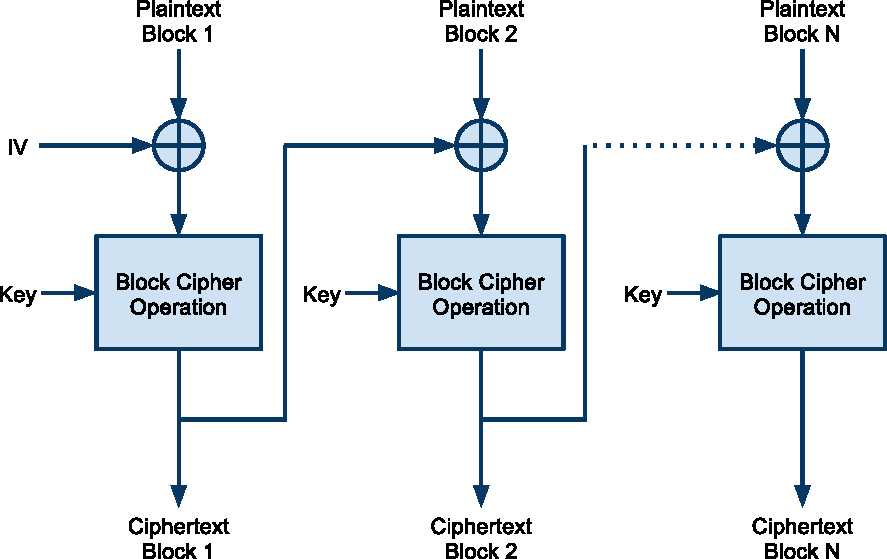
\includegraphics[scale=0.8]{CBCMode.pdf}
    \caption{An illustration of the CBC mode of operation}
    \label{fig:cbc}
\end{figure}

\paragraph{Asymmetric-key Encryption} Asymmetric-key encryption is an
encryption scheme where different keys are used for encryption and decryption
\cite[p. 259]{stallings}.

An asymmetric-key encryption scheme is often called a \emph{public-key
encryption} scheme, where one key is defined as private and the other as
public.  The public key is shared to allow other parties to encrypt messages
that only the owner of the private key can decrypt.

The downside of an asymmetric compared to a symmetric cipher is that it
requires a larger key, and that it has a larger computational overhead to
obtain the same level of confidentiality \cite{schneier}. The probably best
known asymmetric cipher is \ac{RSA}.

\subsection{Cryptographic Hash Functions}

A cryptographic hash function is a deterministic mathematical procedure, which
takes an arbitrary block of data and outputs a fixed size bit string. The
output is referred to as the \emph{hash value}, \emph{message digest} or simply
\emph{digest}.

Another property of a cryptographic hash function, is that the
smallest change in the input data, e.g. one bit, should completely change the
output of the hash function. In other words, it should be infeasible to find the
reverse of a cryptographic hash function \cite[p. 335]{stallings}. It should
also be infeasible to find two blocks of data which produce the same hash
value, i.e. a \emph{collision}.

The standard defined by \ac{NIST} for cryptographic hash functions today, are
\ac{SHA}-1 and the \ac{SHA}-2 family \cite{SHA-FIPS}.


\subsection{MAC Functions}

\citet{schneier} defines a \ac{MAC} to be a construction that detects tampering
with a message -- i.e. it authenticates the message. A \ac{MAC} can be
constructed in different ways. One example is H\ac{MAC} which constructs the
\ac{MAC} using a secret key, the message and a hash function \cite{rfc2104}.

\subsection{Key Derivation Functions}
\label{sec:PBKDF2}

A key derivation function is a function which takes a key, a password, a
passphrase or similar, and creates a new key from it. One of the applications
of such a function, is to create a stronger key from a weaker key, such as a
password. This technique is called \emph{key stretching}. The process involves
making the derivation of a key from a password an expensive process in terms of
computing power, which in turn makes it more resistant to brute force attacks.

\ac{PBKDF2} is a key derivation function that utilizes key stretching. It uses
a password, together with a randomly generated salt and a pseudorandom function
\cite{rfc2898}. The function will combine these inputs in a specific way, and
can repeat the process for a specified number of times, called the
\emph{iteration count}. A higher iteration count results in a stronger key. The
salt provides defence against a precomputed collection of keys, i.e. a
\emph{rainbow table}, in the sense that it will make sure that a password will
not derive the same key if different salts are used.

\subsection{Digital Signatures}

A digital signature is the digital equivalent of a normal signature, i.e. it
verifies that an entity approves with or has written a message. It can also
verify the date the signature was made. In addition, it should be verifiable by
a third party \cite[p.  379]{stallings}. A digital signature should not be
feasible to fake.

The \ac{RSA} cipher can be used to generate signatures. In addition, there is
also a standard for digital signatures defined by \ac{NIST}, called
\ac{DSS}\cite{DSS-FIPS}.  \ac{DSS} uses \ac{DSA} as the underlying algorithm.

\subsection{Digital Certificates and PKI}

A digital certificate is the pairing of a digital signature and a public key
\cite{stallings}. By this scheme, the services confidentiality, authentication
and non-repudiation can be achieved.

For example, a person has a certificate with some clues about an identity in
it, e.g. an e-mail, together with a public key. This certificate can then be
signed using digital signatures, to verify that some other entity trusts this
certificate.

In practice, the entity which signs certificates is the \ac{CA}, which all
clients have the public key information for, and trusts. This is refered to as
a \ac{TTP}. The \ac{CA} will also contain information about which certificates
has been revoked, i.e. should not be trusted in use. Such a scheme is usually
referred to as a \ac{PKI}.

\subsubsection{PGP}

\ac{PGP} is a scheme similar to \ac{PKI}, but with no \ac{CA} that all users
trust \cite{stallings}. Instead, trust is made between users by somehow
verifying their public keys, for instance by meeting face to face. A user can
then sign the key of another user, set a trust level for the user, and publish
this information to a key server. Other users can then calculate a trust on an
unknown person, based on the trust set by people that they trust, from
information located on publicly available key servers.

\subsection{SSL/TLS}

\ac{TLS}, and its predecessor \ac{SSL}, are technologies for obtaining
confidentiality, integrity and authentication for transfer of files over a
network \cite{stallings}. It does so by a combination of different algorithms
and primitives, and a digital certificate is required for authentication.

To transfer files securely over \ac{HTTP}, \ac{TLS}/\ac{SSL} is used to form
\ac{HTTPS}.

\section{Research on Security in Cloud Computing}
\label{sec:research}

This section will elaborate on selected research concerning privacy within
cloud computing. The review of this subject will focus on solutions that
provide confidentiality within the cloud. Solutions that partially provide
privacy are not considered as they are not relevant to our research.

We choose to present the following papers as they provide possible solutions to
the same problems handled in this thesis, although with a different approach.
The first three security systems seek to secure the cloud server itself, and
the last one argues for building a secure system on top of a non-trusted cloud
provider.

\subsection{Privacy as a Service}

A concept entitled \ac{PasS}, was suggested in 2009 \cite{PasS}. \ac{PasS} is a
set of security protocols ensuring privacy of customer data in cloud computing
architectures. The main design goal with \ac{PasS}, is to maximize the user's
control over her sensitive data, both processed and stored within a cloud.

The \ac{PasS} concept is based on a fundamental \emph{system model} and
\emph{trust model}. The system model consists of three communicating parties,
namely a \emph{cloud provider}, a \emph{cloud customer} and a \emph{\ac{TTP}}.
The \ac{PasS} system model is shown in Figure \ref{fig:RW:PasS}.

\begin{figure}[h!]
    \centering
    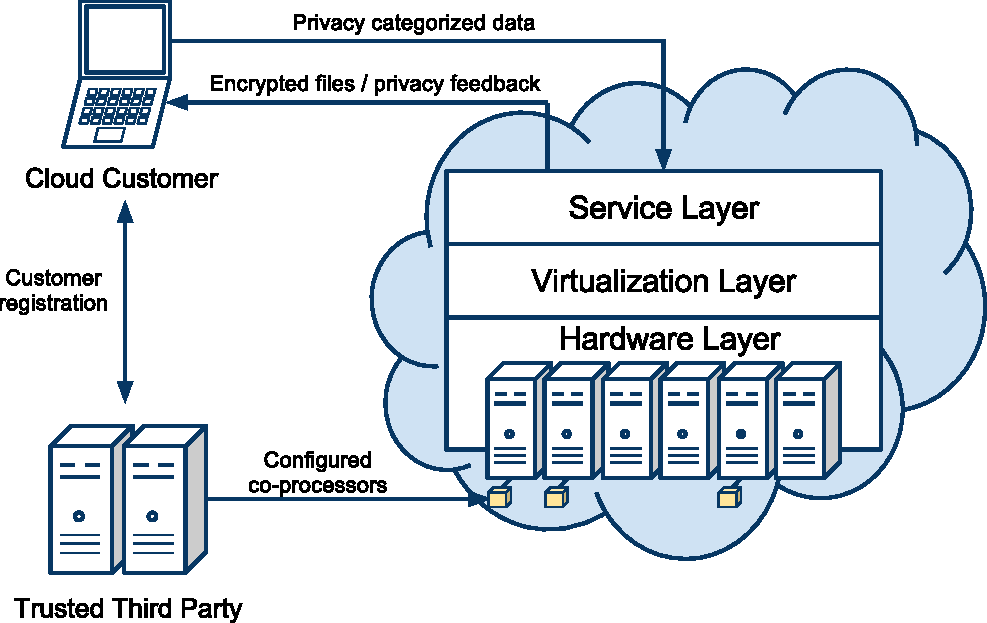
\includegraphics[scale=0.6]{ArchitecturePasS.pdf}
    \caption{System model of PasS}
    \label{fig:RW:PasS}
\end{figure}

It is important to notice that the \ac{PasS} system model is dependent on
pre-installed cryptographic coprocessors in the hardware running the cloud
service. A cryptographic coprocessor is in this context defined as a small
hardware card, including a processor, \ac{RAM}, \ac{ROM}, backup battery,
persistent storage and an Ethernet network card. A coprocessor interfaces with
a server in the cloud, and provides a safe environment for processing of
customer's data.

The cryptographic coprocessors are used in the cloud because they are
supposedly tamper-proof against physical attacks. The coprocessors are
preconfigured by the \ac{TTP} before they are installed. By using this
procedure,a safe computational environment for the cloud customer is provided,
which is kept secret from the cloud provider.

The main task of the \ac{TTP} is to compute a set of public/private key pairs,
load them into the persistent storage of the coprocessor, and further send
them to the customer. The \ac{TTP} also loads its own secret key into the
coprocessor. This key distribution ensures secure communication between the
three parties. The key pair of the customer is sent through a secure
communication channel.

With cryptographic coprocessors in the cloud and a secure communication, the
cloud customer can choose between three different levels of privacy towards the
cloud provider -- no privacy, privacy with a trusted provider and privacy with
a non-trusted provider.

\emph{No privacy} implies storing data as clear text in the cloud.
\emph{Privacy with a trusted provider} involves storing encrypted data in the
cloud. This data is encrypted by the cloud provider and only achievable by the
customer or cloud provider.

In the case of \emph{privacy with a non-trusted provider}, the customer
encrypts the private data before uploading it to the cloud provider. The key
used for encryption is shared with the cryptographic coprocessor, through an
authenticated version of the Diffie-Hellman key management protocol. The
coprocessor can further process the encrypted data and store it in the cloud
facility. The stored data is encrypted and unknown to the cloud provider.

\subsection{Privacy Manager}

In 2009, HP Labs proposed a way to manage and control the private data of
users, stored and processed in a cloud facility \cite{privacymanager}. Their
solution was partially implemented as a software program called \emph{privacy
manager}.

The privacy manager uses a feature called \emph{obfuscation}, which is similar
to encryption. However, the obfuscation method is different from encryption in
the sense that the obfuscated data can be processed in the cloud, without the
cloud provider knowing the encryption key or the original data.
\citet{privacymanager} mention the following obfuscation methods:

\begin{itemize}
\item Yao's protocol for secure two-party computation \cite{yao}
\item Gentry's homomorphic encryption scheme \cite{gentry}
\item Narayanan and Schmatikov's obfuscation method \cite{obfuscationmethod}
\end{itemize}

Due to better efficiency, the privacy manager uses the latter alternative.
However, the obfuscation method of Narayanan and Schmatikov does not provide
complete confidentiality to the cloud provider \cite{obfuscationmethod}.

In addition to installing a privacy manager at the user's terminal, HP Labs
suggests the use of trusted computing solutions to address the lower-level
protection of data. The
\ac{TCG}\footnote{\url{http://www.trustedcomputinggroup.org/}} is an example of
an organization developing and providing trusted computing solutions. A
tamper-proof piece of hardware called a \ac{TPM} is recommended
\cite{privacymanager}, which is designed by \ac{TCG}. The \ac{TPM} is installed
in the machine running the privacy manager, to ensure that processes carried
out by the privacy manager can be fully trusted.

The privacy manager is suggested to work in three different use cases. It can
be implemented to support a \emph{single client}, the use of \emph{hybrid
clouds} and/or the use of an \emph{infomediary} within the cloud.

%Regarding applications in the cloud where users have to upload unobfuscated
%private data, the privacy manager includes two additional features called
%preferences and personae. Both features are dependent on a trustworthy service
%and cloud provider, and are therefore irrelevant to our development.

\subsection{Trusted Cloud Computing Platform}

Equal to \acl{PasS} and the privacy manager, \emph{\ac{TCCP}} was proposed as a
solution to provide secure computations and storage within a non-trusted cloud
provider \cite{tccp}. As opposed to the previous solutions, \ac{TCCP} is
directed against secure execution of guest \acp{VM} outsourced to \ac{IaaS}
providers.

The original infrastructure, before adding \ac{TCCP}, is assumed to
consist of a \emph{cloud manager}, which manages a cluster of nodes running one or more
\acp{VM}. Among multiple tasks, the cloud manager is responsible for loading \ac{VM}
images into its own nodes.  Each node has a \emph{\ac{VM} monitor} which will further
launch and monitor \acp{VM} from the received corresponding images.

\ac{TCCP} is based upon the \ac{TPM} chip and is a \emph{remote attestation
scheme}.  The scheme enables a network entity to verify whether another remote
entity runs a \ac{TPM} chip or not.

The \ac{TCCP} system architecture is illustrated in Figure \ref{fig:RW:TCCP}.
The trusted computing base of \ac{TCCP} includes a \emph{trusted coordinator}
and a \emph{trusted virtual machine monitor}. The coordinator manages the
trusted nodes within a cluster. To be trusted, a node must be located within a
security perimeter and run a trusted virtual machine monitor.

\begin{figure}[h!]
    \centering
    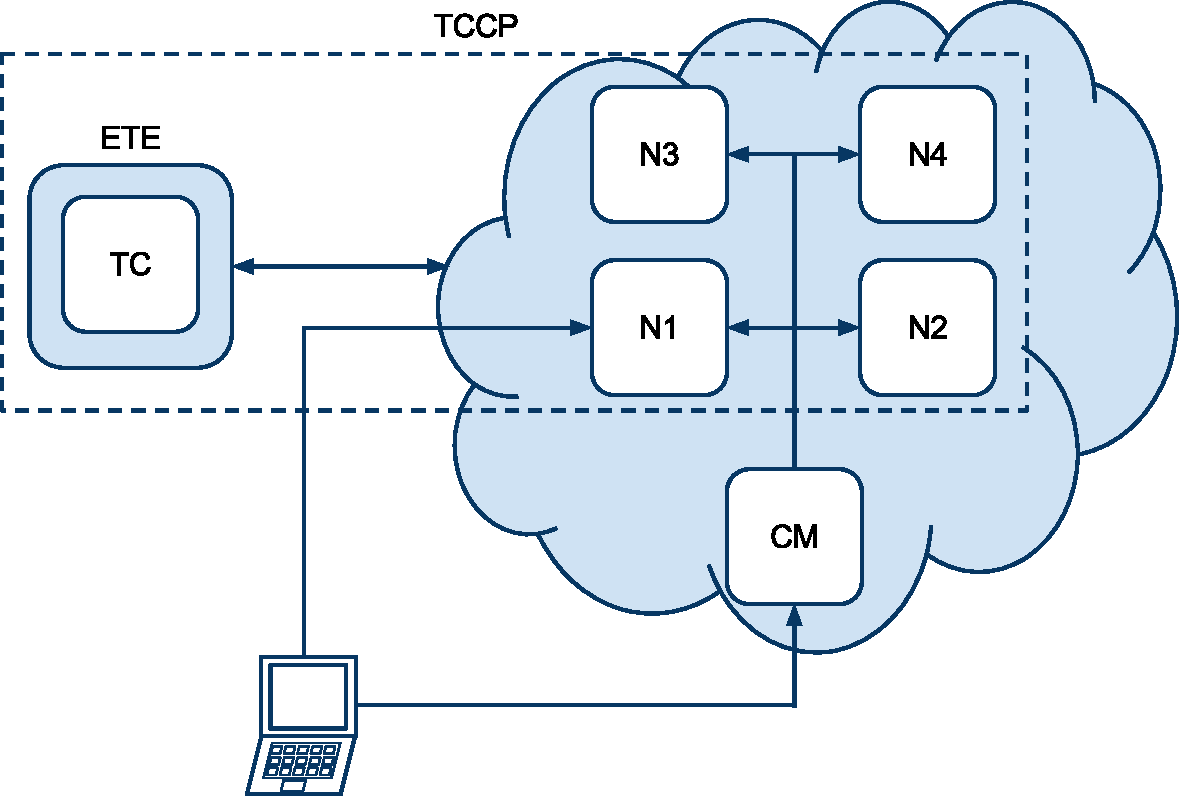
\includegraphics[scale=0.4]{ArchitectureTCCP.pdf}
    \caption{System architecture of TCCP}
    \label{fig:RW:TCCP}
\end{figure}

The coordinator maintains a record of the nodes located in the security
perimeter, and use remote attestation to ensure nodes are trusted. Each trusted
node in a cluster contains a \ac{TPM} chip and a corresponding trusted monitor.
The main task of the trusted monitor, is to enforce a local closed box
protection of a client's running \ac{VM}.

Each trusted virtual machine monitor cooperates with a trusted coordinator to
protect the transmission of \acp{VM} between trusted nodes, and to ensure that
\acp{VM} are executed by trusted nodes. In this context, the \ac{TCCP}
specifies several protocols for both launching and migrating \acp{VM} inside
the cloud. These protocols are described by \citet{tccp}.

The trusted coordinator-part is installed in servers operated and maintained by a
trusted third party, to prevent unwanted tampering from the \ac{IaaS} provider.
A client can further use remote attestation to the coordinator to verify that the
\ac{IaaS} provider secures its computation.

With \ac{TCCP}, the client interacts with the \ac{IaaS} provider as usual. The
difference is that the trusted nodes and their trusted coordinator communicates
to ensure a secure environment for executing the client's \ac{VM}.

\subsection{Cryptographic Cloud Storage}

In 2010, researchers at Microsoft were looking at the problem of building a
secure cloud storage service on top of a non-trusted storage provider
\cite{microsoftresearch}. They describe architectural solutions related to both
personal and enterprise use cases. The architectures are explained in high
level and are designed to utilize and combine recent and non-standard
cryptographic primitives. The personal scenario is depicted in Figure
\ref{fig:RW:CCS:CA}.

\begin{figure}[h!]
    \centering
    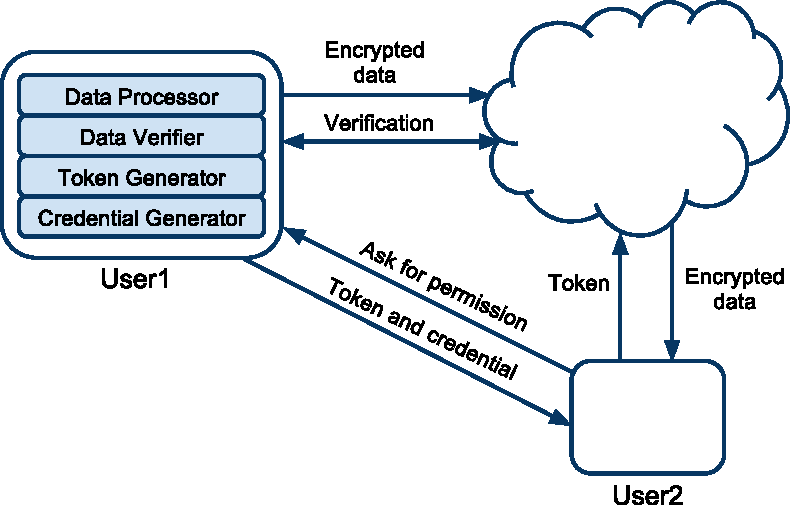
\includegraphics[scale=0.6]{ArchitectureCCSC.pdf}
    \caption{Cryptographic cloud storage, personal scenario.}
    \label{fig:RW:CCS:CA}
\end{figure}

The architecture consists of the following computational components:
\begin{itemize}
  \item Data Processor
  \item Data Verifier
  \item Token Generator
  \item Credential Generator
\end{itemize}

The Data Processor is responsible for encrypting data before it is sent to the
cloud, and decrypting data when it is retrieved.

Integrity is supported through a Data Verifier component, which checks whether
specific data has been tampered with. The verification procedure is independent
of the download and upload procedures, and can be called at any time by the
user.

The Token Generator is used by the user to generate tokens that works like
data identifiers. Tokens are given to and utilized by the provider to
find data requested.

To enable sharing of data, the architectural scheme is suggested to use a
Credential Generator. The Credential Generator is responsible for generating
and sending credentials to other users. These credentials are cryptographic
keys that can be used to decrypt defined portions of data. The user must also
send the corresponding tokens together with the credentials to share data. How
tokens and credentials are sent between users is not discussed.

\paragraph{Attribute Based Encryption} Microsoft propose to utilize
\emph{attribute based encryption} for confidentiality. In attribute based
encryption, data is encrypted using a public key and series of attributes
defined as a \emph{policy}. This ciphertext can further be decrypted by a set
of decryption keys. A decryption key is associated with a set of attributes,
and is able to decrypt the ciphertext if it contains a given number of the
attributes used to encrypt the ciphertext \cite{microsoftresearch}. The private
keys are meant to be implemented as the distributed credentials mentioned
above.

It is important to mention that attribute based encryption is a relatively new
technique in cryptography, which can make it hard to define its level of
security.

\paragraph{Proof of Storage} The verification procedure is proposed to utilize
a proof of storage protocol to provide integrity. The protocol utilize small
portions of information independent of the size of the verified data and can be
executed an arbitrary number of times. Applicable protocols for proof of
storage are defined in \cite{proofofstorage1, proofofstorage2}.

\paragraph{Enterprise Scenario} The solution for an enterprise scenario is
similar to the one of a regular user, however computational components are
rather dedicated to separated machines to provide scalability. The suggested
architecture for an enterprise scenario is shown in Figure \ref{fig:RW:CCS:EA}.

\begin{figure}[h!]
    \centering
    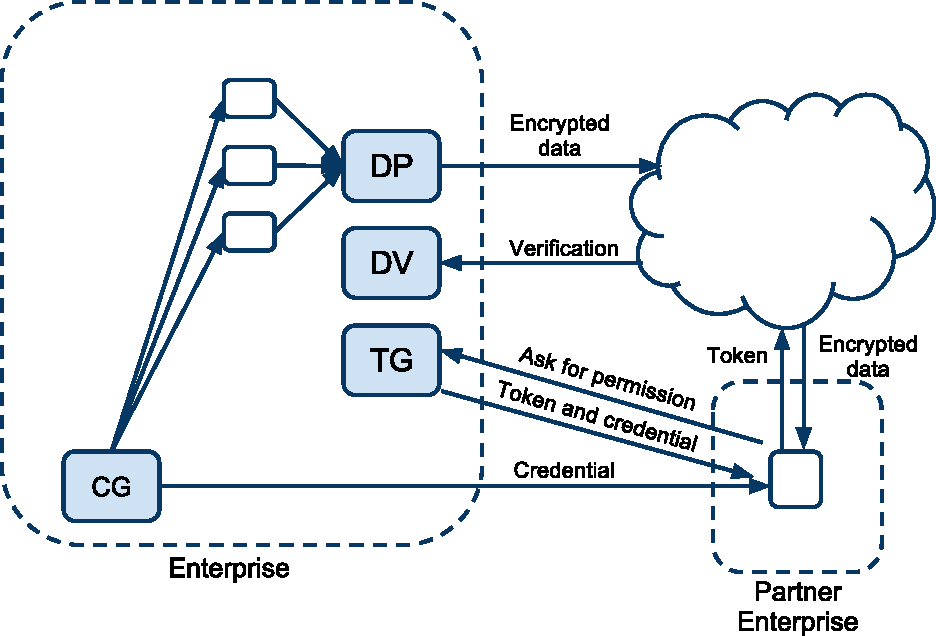
\includegraphics[scale=0.6]{ArchitectureCCSE.pdf}
    \caption{Cryptographic cloud storage, enterprise scenario.}
    \label{fig:RW:CCS:EA}
\end{figure}

It is important to notice that each employee will need an initial credential
from the credential generator to use the cloud storage application. The
distribution of these credentials is not discussed.

\section{Existing Solutions}
\label{sec:existing}

There are a number of existing solutions for storing data in the cloud,
with more or less the functionality required to fulfil the problem
description for this thesis. The section highlights some of them.

\subsection{Dropbox}

Dropbox\footnote{\url{http://www.dropbox.com/}} is a popular commercial
application for storing data in the cloud, claiming more than 25 million users
\cite{dropbox_users}. All files are saved using Amazons S3 storage service.

The company claims the use of strong encryption and strict access control
\cite{dropbox_security}, but has received criticism for its lack of security
\cite{dropbox_concerns}. Among these concerns, is the \emph{Forgotten Password}
feature, that enables Dropbox to hold the passwords of their users. This
implies that the encryption is performed server-side and that Dropbox can read
all data stored with their service.

In addition, Dropbox is not open source, and hence it is difficult to verify
that the security features actually work as claimed.

\subsection{Tahoe-LAFS}
\label{sec:tahoe}

Tahoe-\ac{LAFS}\footnote{\url{http://www.tahoe-lafs.org/}} is an open source,
distributed and secure cloud storage file system, fulfilling the criteria in
Section \ref{sec:criteria}. The integrity and confidentiality of the
files are guaranteed by the algorithms used on the client, and is independent
of the storage servers, which may be operated by untrusted people.
This is defined as \emph{provider-independent security} \cite{tahoe}.

In Tahoe-\ac{LAFS}, files are exclusively encrypted client-side, then split up
using \emph{erasure coding}, before being uploaded to the cloud, as illustrated
in Figure \ref{fig:B:tahoe}.

\begin{figure}[h!]
    \centering
    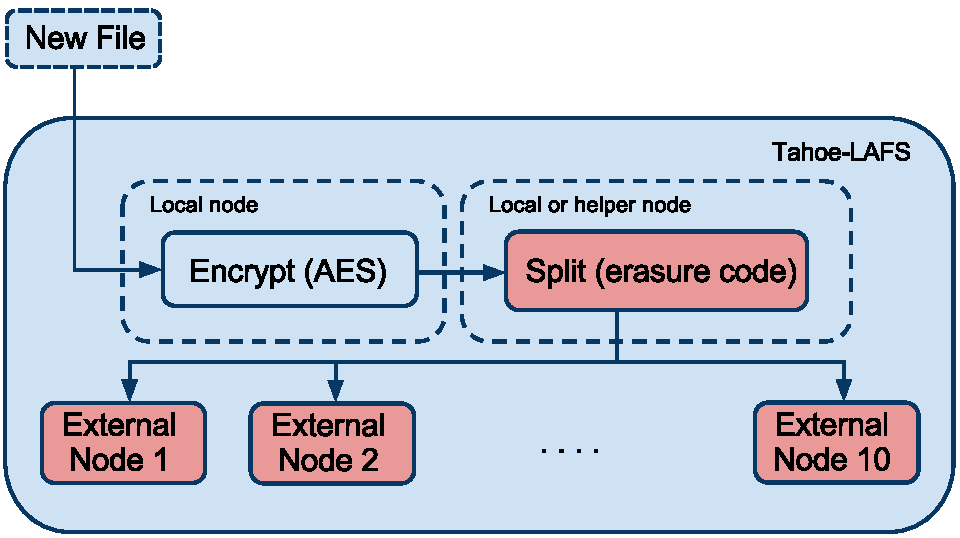
\includegraphics[width=\columnwidth]{Tahoe-newfile.pdf}
    \caption{Tahoe-LAFS: Insertion of a new file}
    \label{fig:B:tahoe}
\end{figure}

\subsubsection{Architecture of Tahoe-LAFS}

Tahoe-\ac{LAFS} has a three layer architecture: the key-value store, the file
system, and the application \cite{tahoe}.

The \emph{key-value store}, is the lowest layer and is implemented by a grid of
Tahoe-LAFS storage servers. Data is kept on the storage servers in the form of
\emph{shares}, which are encrypted and encoded parts of files.
\emph{Capabilities} are short ASCII strings, containing information on where to
find, decrypt and verify a file or folder. Nodes in the grid learn about each
other through an \emph{introducer}.

The \emph{file system} layer is responsible for mapping human-meaningful
pathnames to pieces of data. Each directory contains a table of capabilities
for its children, i.e. subdirectories or files. Two main forms of capabilities
are available for each file, read-only and read-write, and these can be
distributed to e.g. share a file with friends.

Since it is not practical for users to remember strings containing random
characters, the \emph{application} layer is used for providing a user-friendly
interface to the directories and files.

\paragraph{File Types} There are two kinds of files in the Tahoe-\ac{LAFS} --
\emph{immutable} and \emph{mutable} files. An immutable file is created
exactly once. Mutable files can be modified, and everyone who has access to the
signing key can make new versions of the mutable file. Directories are
implemented as mutable files.

\paragraph{Erasure Coding} By using the Solomon-Reed erasure coding scheme,
Tahoe-\ac{LAFS} is able to recover a file using only a predefined subset of the
parts distributed to the storage servers. Erasure coding is a type of \ac{FEC}
code, which extends a message with $C$ characters into a longer message with
$N$ symbols \cite{t_reed-solomon}. The original $C$ characters can then be
recovered from a subset of the $N$ symbols.

\paragraph{Sharing} To share a folder, and hence its subfolders and files, the
corresponding capability of the folder has to be distributed. Tahoe-\ac{LAFS}
in itself does not provide a specific way of doing this, and leaves it up to
the user to distribute keys in a secure manner.

\subsection{Wuala}

Wuala\footnote{\url{http://www.wuala.com/}} is a software offering a secure
cloud storage file system. It is written in the Java programming language, and
hence has easily been ported to a number of platforms, e.g. Windows, Linux, OS
X and Android.

\paragraph{Sources of Information} The authors have released a paper on a
cryptographic tree structure for the file system that Wuala uses, called
Cryptree \cite{cryptree}, but other details of how the system works is hard to
come by. The only source of technical information of this system found, was a
Google Tech Talk \cite{wuala}.

A side from this, Wuala is closed source, and hence it is difficult to verify
that the software indeed does what it states.

\paragraph{Network Scheme} Wuala claims strong focus on reliability and
availability, by both providing storage on their own central servers, in
addition to a \emph{\ac{P2P} cloud} of Wuala users that has donated capacity to
the system. There are also additional advantages resulting directly from using
a distribution scheme based on \ac{P2P}.  Examples of this are no maximum file
size and no traffic limit.

Similar to the Tahoe-\ac{LAFS}, Wuala uses an erasure coding scheme in the
family of Reed-Solomon \cite{wuala} to enable the logic behind splitting and
combining parts of a file and creating redundancy.

\paragraph{Sharing} Files and folders can be either \emph{private},
\emph{shared} or \emph{public}. In addition, there exist a concept of public
and private \emph{groups} of users, which can be used to manage access control
over shared folders and files.

When creating a new group in the Wuala client, as depicted in Figure
\ref{fig:wuala:newgroup}, the default choice is to create a private group, but
provide access through a \emph{secret link} via the Wuala web page.
This implies a key distribution where the group members has to rely on Wuala as
a trusted third party.

\begin{figure}[h!]
    \centering
    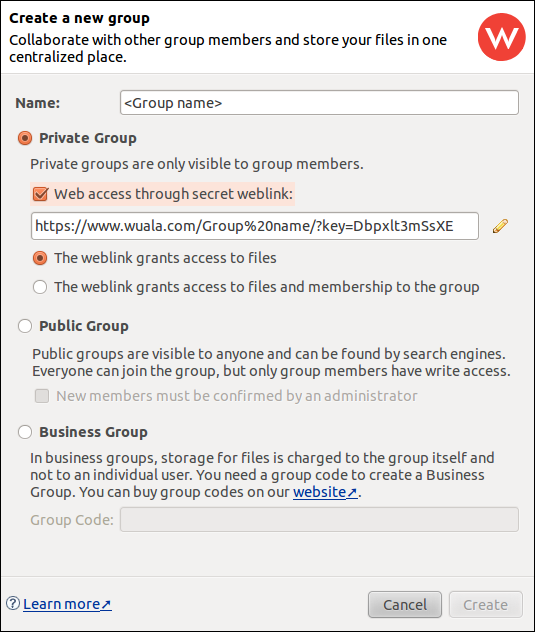
\includegraphics[width=\columnwidth]{wuala_create_group.png}
    \caption{Creating a new group in Wuala}
    \label{fig:wuala:newgroup}
\end{figure}

\paragraph{Security} When adding a new file to Wuala, the file and its meta
data are encrypted with 128 bit \ac{AES}, before encoded into redundant
fragments using erasure codes, and lastly uploaded to the network. 2048 bit
\ac{RSA} is used for authentication. All cryptographic operations are performed
locally on the client-side, and the password used never leaves the client.

Access control are provided using the efficient cryptographic tree structure
Cryptree \cite{cryptree, wuala}, which is based on the notion that no
information should be revealed to the computer holding the access control
structure, i.e. the hosting server or the \ac{P2P} network. Keys for nodes in
the tree are derived from the keys of the parents, implying that if a user has
a key to a folder, she also has access to all the subfolders and files.

However, since the source of Wuala is not available for scrutiny by the public,
none of these security features can easily be verified.

%**************************************%
\chapter{Technical Procedure}
\label{ch:technical}
%**************************************%

This chapter will describe our architectural and cryptographic
scheme for providing secure storage of data on a remote untrusted system. It
will further explain the procedures carried out to create a proof of concept
application, that implements the proposed architectural and cryptographic
scheme. The application, named \emph{\ac{CSV}}, is implemented as an Android
application, and consists of separate server and client functionality.

The chapter will start by giving an overview of the proposed architecture
followed by a more detailed description of the corresponding cryptographic
scheme. The chapter will end by describing the implementation details for both
the server and client-side functionality of the Cloud Storage Vault.

\section{Architectural Overview}
%**************************************%
\label{chap:AS}

The architectural solution of a secure cloud file sharing system has to
convince its users that the functions indeed are secure, and that the concepts
are easy to understand and accept. The following sections will elaborate on the
architecture, favouring simplicity and familiar concepts, such as files and
directories. We also introduce the concept of \emph{capabilities}. Key concepts
are based on equivalent operations found in Tahoe-\ac{LAFS} \cite{tahoe}.

Figure \ref{fig:AS:overview} represents an overview of the functionality that
the architecture must support. The illustration exhibits a user uploading a
file to the cloud, and adding this to a parent directory. After she has done
this, it is possible for her to distribute the capability of the file to other
users to realize sharing of files or directories.

\begin{figure}[h!]
    \centering
    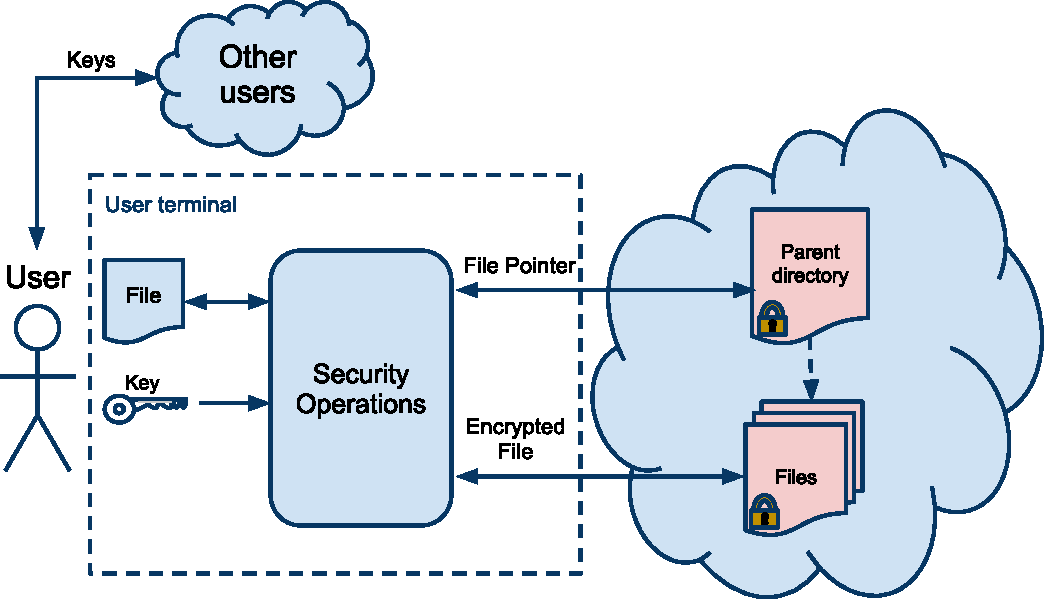
\includegraphics[width=\columnwidth]{ArchitectureOverview.pdf}
    \caption{Overview of user functionality}
    \label{fig:AS:overview}
\end{figure}

\subsection{File Storage}
\label{sec:AS:FS}

The solution for file storage proposed in this thesis, is that only a simple
\emph{key-value store} is needed on the server-side. The key works as a lookup
index for a specific value, while the corresponding value equals an encrypted
file object. The server will be required to support the operations of uploading
and downloading key-value pairs to this store.

From the users perspective, a file object can have multiple forms -- it can
either be a \emph{mutable} or an \emph{immutable} file. A mutable file can be
changed, and is what a user will see as a directory, while an immutable file is
as a normal file but cannot be changed.

A user will need certain information to be able to reach and read a file
object, and we define these properties as the \emph{capability} of a file
object.  For now, the capability represents the ability to find, read, verify
that a file has not been tampered with, and write to a mutable file.

Both the concept of two different file types, and capabilities are influenced
by the similar use in Tahoe-\ac{LAFS}.

\subsubsection{Directory Structure}

The contents of a directory are files and other directories. More specifically,
a directory contains the means to find files or directories, namely the
corresponding capabilities. In addition, there exist a human readable name, an
\emph{alias}, for each entry in a directory. This design gives a flexible and
space-conservative structure, since any file object may be found in multiple
directories, but does only exist once in the cloud.

A user will need to have some way of storing the capabilities of her file
objects. This could potentially be done client-side, but a problem arises if
the user wants to use several terminals. Thus, we introduce the \emph{root
folder}, a folder from which all other files and folders can be reached. The
user will only need to know of one single capability to reach all her stored
data. This capability has to be stored in a secure manner, e.g. in an
\emph{encrypted keyring}. The resulting structure is a directed graph, as
illustrated in Figure \ref{fig:AS:filesystem}.

\begin{figure}[h!]
    \centering
    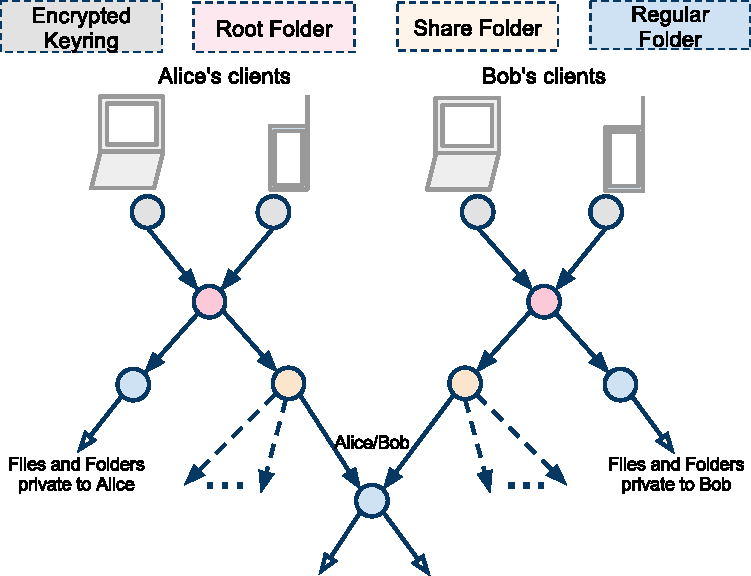
\includegraphics[width=\columnwidth]{ArchitectureFileSystem.pdf}
    \caption{File system structure}
    \label{fig:AS:filesystem}
\end{figure}

\subsection{Authorization, Authentication and Accounting Layer}
\label{sec:accounting}

The possession of a capability gives a user access to read a file or read or
write a folder, and hence serves as the primary access control. There are
however some properties that the server provider might want that cannot be
given by the capability. Therefore a layer implementing authentication,
accounting and authorization might be preferable.

\subsubsection{Block Access to Encrypted Data}

The capability for a file or folder might be intentionally or unintentionally
leaked by a user. In this case, it would be preferable that the server can
block access to a particular object. The server could also potentially enforce
access rights on all encrypted objects, so that they are only retrievable by
the owner. This would however complicate sharing.

\subsubsection{Modification and Deletion of Files}

For each directory, there exist a different capability for read and write
operations, though the read capability can be deduced from the write
capability. From the write capability, it is possible to deduce another secret,
the \emph{write enabler}, which the server also knows of.  Knowledge of the
write enabler is needed for the server to grant access to modify or possibly
delete a folder.

For immutable files, there is no concept of write access, only read. A user
might not want to pay for storage of files that she no longer needs.  A layer
that identifies the creator of a file, can by the same method decide who
should have the rights to delete it.

\subsubsection{Accounting}

If the server-side of the system is held by a cloud storage provider, it is
important to be able to decide which users should be billed for the \emph{file
storage} and generated \emph{network traffic}.

In the case of an immutable file, the storage costs can be billed to the user
creating the file. The costs of network traffic can further be charged to the
users retrieving the file.

Accounting might also be interesting for an organization using a third party
cloud provider. For instance an employee who leaves the organization, might be
tempted to copy all the data stored on the server. The organization should then
be able to discover what has been done, using some form of an audit trail.

It is however worth noting that if the accounting happens server-side, there is
no real way to verify that all logs stored there are correct, since the cloud
provider will have access to modify or delete them.

\subsection{User Scenarios}

The various user scenarios supported by the software, provides a logical way to
describe the external properties of the system. The fundamental operations are
\emph{downloading}, \emph{uploading} and \emph{sharing} of files and folders.

\subsubsection{Download File}

The download procedure is depicted in Figure \ref{fig:AS:download}. The client
sends a download request with the identifier of a folder, which she possesses
the capability of. The server will respond with the encrypted directory.
The user will use the capability to decrypt the directory.

\begin{figure}[h!]
    \centering
    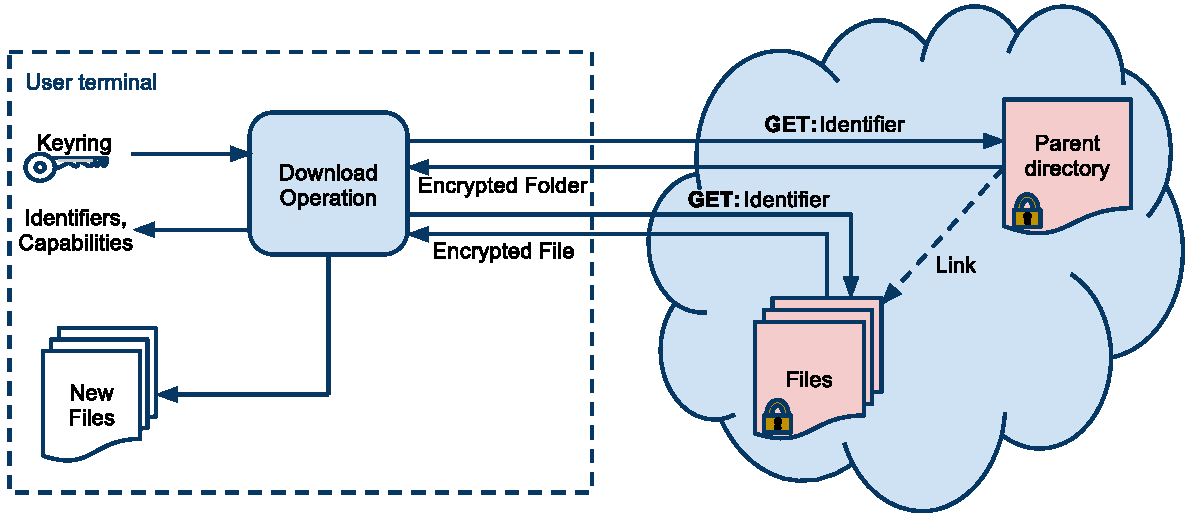
\includegraphics[width=\columnwidth]{ArchitectureDownload.pdf}
    \caption{Scenario: Downloading a file}
    \label{fig:AS:download}
\end{figure}

In the directory, the user finds the aliases and necessary capabilities to gain
access to the children of that folder. If the user now wants to download a file
from the accessed folder, she obtains the identifier from the capability, and
requests the server for this file. Once downloaded, the capability provides
means of decrypting and verifying that the data has not been tampered with.

\subsubsection{Upload File}

Figure \ref{fig:AS:upload} shows the process of uploading a new file. The
capability is generated by the client, and used to encrypt the data. The file
is then uploaded to the server, and the capability and an alias is linked in to
the parent folder.

\begin{figure}[h!]
    \centering
    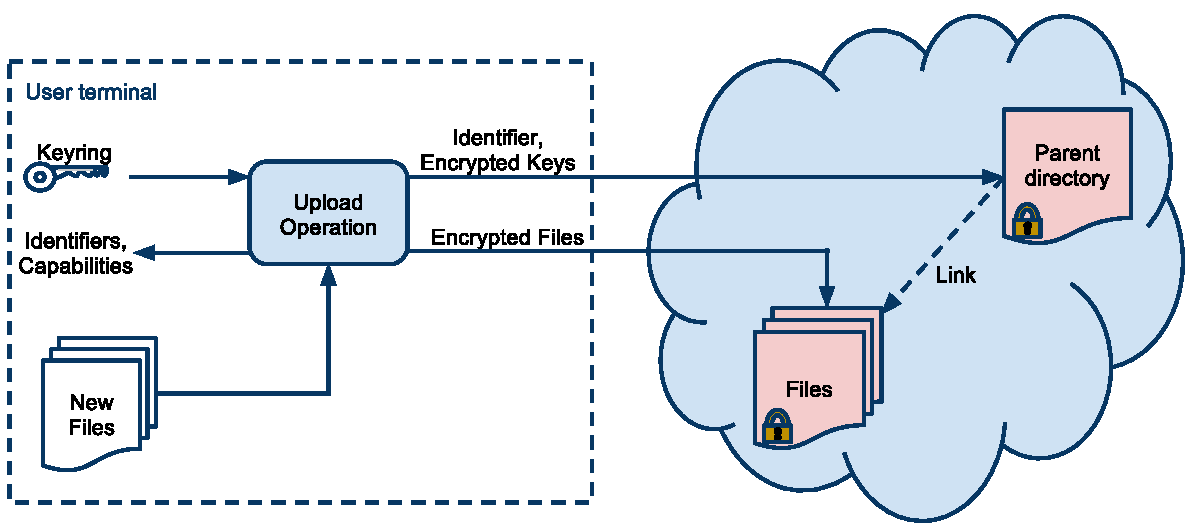
\includegraphics[width=\columnwidth]{ArchitectureUpload.pdf}
    \caption{Scenario: Uploading a file}
    \label{fig:AS:upload}
\end{figure}

\subsubsection{Share Files}

As shown in Figure \ref{fig:AS:sharing}, for Alice to be able to share files
with Bob, she first has to create a new directory that will contain these
files. Alice is then required to share the capability of the new directory with
Bob. When the capability is shared, the new directory will work as a secure
channel where Bob and Alice can share their own folders and files.

\begin{figure}[h!]
    \centering
    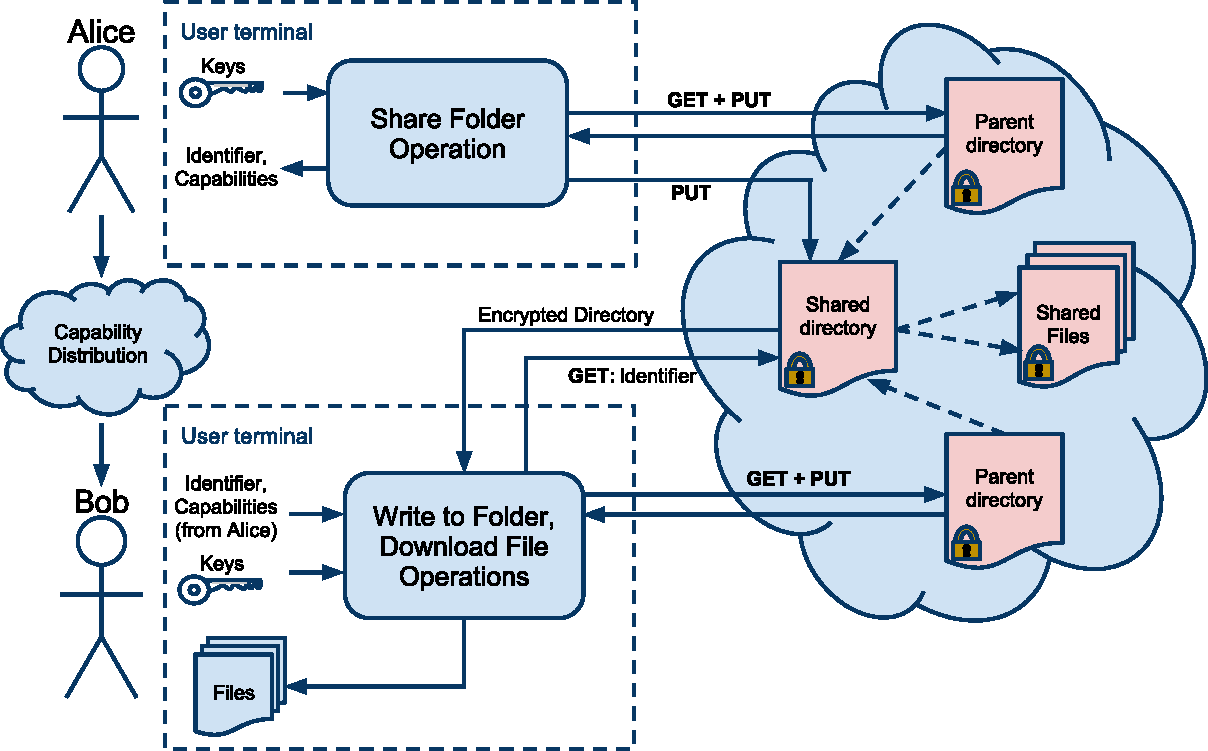
\includegraphics[width=\columnwidth]{ArchitectureShare.pdf}
    \caption{Scenario: Alice shares a file with Bob}
    \label{fig:AS:sharing}
\end{figure}

Before transferring the capability to Bob, Alice links the shared directory
to a parent directory, so she can easily retrieve it at a later time. She can
also link files and other directories to the shared directory.

The capability distribution is a key design issue, and has to be performed in a
secure manner. This can be solved in a variety of ways, and the solutions
proposed in this thesis are discussed in Section \ref{sec:DI:keydist}.

After receiving the capabilities for the shared folder from Alice, Bob requests
and receives the encrypted shared directory, in addition to linking it with a
parent directory for future usage. He can then download shared files as if they
were his own.

\paragraph{Read-Only Shares}

If Alice wants to share a directory in read-only mode, she can simply share the
read capability with Bob, instead of the write capability. This will work as
intended, but might prove somewhat cumbersome for Alice. If Alice wants to
write to the directory she has shared with Bob, she cannot enter it through
the parent folder shared with Bob, since this will only grant her the read
capability. The implication is that Alice will have to access the directory
through another path in her directory tree, to get the write capability.

A more simple solution is to enable Alice to store the write capability
individually among her private files, while storing the read capability in the
shared parent directory. The solution can easily be implemented by using a
specialized \emph{write key folder} under Alice's root folder. The write key
folder will then contain write capabilities to every folder that Alice has
shared in read-only mode. The idea behind the write key folder is illustrated
in Figure \ref{fig:AS:readonly}.

\begin{figure}[h!]
    \centering
    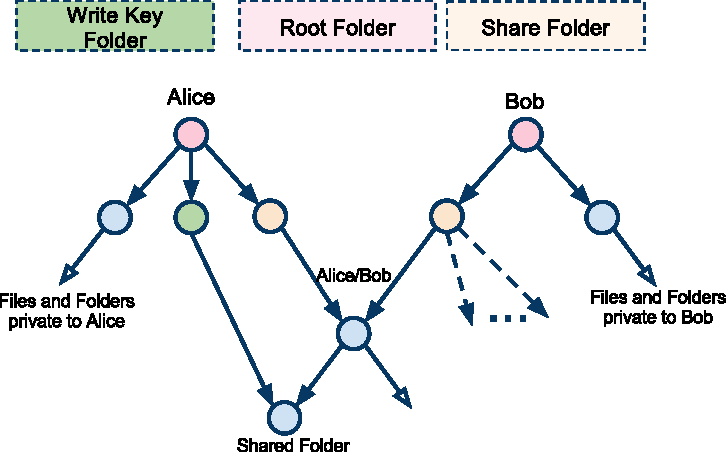
\includegraphics[width=\columnwidth]{ArchitectureShareReadOnlyFolder.pdf}
    \caption{Sharing read-only folders}
    \label{fig:AS:readonly}
\end{figure}

\subsection{Constraints}

The software using this architecture should be able to run on restricted
devices, i.e. equipment with limited memory and \ac{CPU} power, often in
addition to constraints on power and network utilization. This has implications
for the design of the software, since all cryptographic operations has to be
performed client-side.

%**************************************%
\section{Cryptographic Architecture}
%**************************************%
\label{chap:CS}

This section elaborates on the cryptographic solutions applied to the
architecture in Section \ref{chap:AS}. It will take a closer look at
how confidentiality and integrity are solved.

We will start with a brief introduction explaining the fundamental security
concepts. The cryptographic architecture is further described in terms of file
and directory operations.  

\subsection{Security Concepts}

The basic security concept of the application is to keep the files of a user
confidential to a third-party storage provider. To solve this, the application
encrypts data locally at the user terminal before uploading them.

When accessing a file, the application downloads the encrypted file before
decrypting it locally. To enable this simple encryption scheme, the user is
required to possess the knowledge of at least one capability, which contains
cryptographic keys to decrypt and verify the contents of the root folder.

The root folder will in turn contain the capabilities for its own children,
which enables the client to decrypt files and folders stored in the root
folder. The other folders work in the same manner.

By initially knowing that files are placed encrypted on a remote server and
that the user possesses one or more cryptographic keys locally, we can continue
with a more comprehensive description of the complete cryptographic solution.
The details are explained in terms of capabilities and the operations conducted
on files and folders.

\paragraph{Capabilities} Capabilities are containers which has the
necessary information to locate, encrypt, decrypt, verify and possibly write
file objects. The possession of a capability grants these rights, which can be
either read access or read and write access. Such an access scheme is known as
\emph{capabilities as keys} \cite{capabilitymyths}. The contents of a
capability is summarized in Table \ref{tbl:capability}, and will vary somewhat
for files and folders, since they are implemented by immutable and mutable
files respectively.

\begin{table}
  \centering
  \caption{The structure of a folder entry}
  \begin{tabular}{ | l | l |}
    \hline
    \textbf{Data}       & \textbf{Comment}                          \\ \hline
     Alias              & Human readable name of file/folder        \\ \hline
     Storage Index      & Key to retrive file/folder from server    \\ \hline
     Write Key          & Only for folders, needed to write a file  \\ \hline
     Read Key           &                                           \\ \hline
     Verify Key         & Only for folders, needed to verify a file  \\ \hline
  \end{tabular}
  \label{tbl:folder:contents}
\end{table}


\paragraph{Encrypted Keyring} Every user will need to possess a root capability
to access their files. Due to the amount and randomness of data in a
capability, it will be impossible for most users to remember. To keep a copy of
the capability on the user terminal is a possible solution, but since such a
device could be lost or stolen it should be protected in an encrypted keyring.
This keyring can then be unlocked by something which the user is able to
remember, such as a password.

\paragraph{Secure Channel} Even though the security of the contents of the
files relies on cryptographic operations performed client-side, a secure
channel between the client and the server has to be formed. This is because of
the possibility for an attacker, Mallory, to do various unwanted procedures if
such a channel is not in place. Firstly, she can discover write enablers, and
thus be able to replace directories. Similarly, Mallory can replay recorded
messages, e.g. to set a folder back to a previous state. By extracting the
username and password, she can also manipulate accounting features by saving
files taking up place in the quota of another user.

\subsection{File and Directory Operations}
\label{sec:CS:DO}

This section describes the elementary file and directory operations supported
by the application. The basic file operations are \emph{upload file} and
\emph{download file}, and correspondingly for directories, \emph{create
directory}, \emph{open directory} and \emph{modify directory}.

For simplicity, the illustrations in the following sections includes naming of
cryptographic primitives. However, it is important to note that this
cryptographic scheme will work with other primitives. Any symmetric cipher
could work instead of \ac{AES}, any signing function that uses both a private
and public key could be used instead of \ac{RSA}, any \ac{MAC} could be used
instead of HMAC-\ac{SHA} and any cryptographic hash function could be used.

The security of the system does rely on these choices, and a recommendation
with rationale for each of the needed primitives will be given in Section
\ref{sec:cryptoprimitivechoice}.

The scheme used for directory operations, are influenced and similar to the one
found in Tahoe-\ac{LAFS}.

\subsubsection{Upload File}
\label{sec:CS:CF}

The operation behind uploading a file, is depicted in Figure \ref{fig:CS:CF}. A
random symmetric encryption key is generated. This is hashed once to obtain the
\emph{storage index}, i.e. the identifier of the file. The storage index is
then hashed again to form the \ac{IV} for the file.

Next, the file is hashed and the resulting digest is stored together with the
encryption key in the capability. Finally, the file is encrypted with the
encryption key and the \ac{IV}, before being transferred to the server.

\begin{figure}[h!]
    \centering
    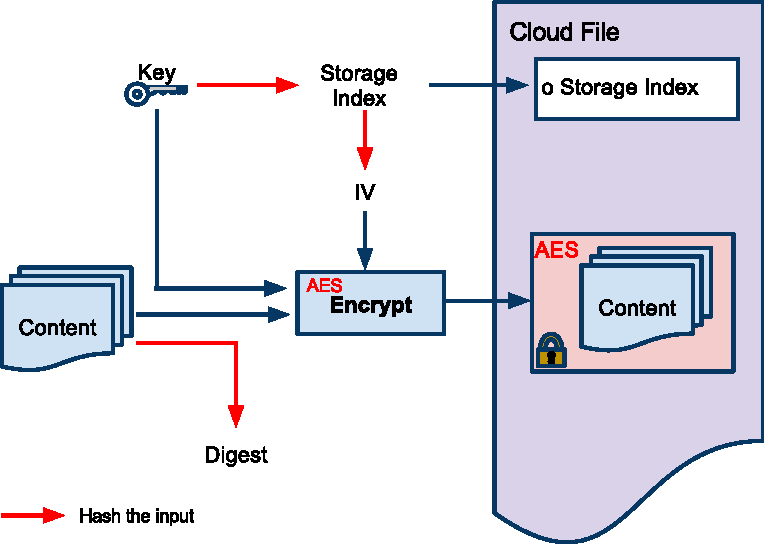
\includegraphics[width=\columnwidth]{CryptoCreateFile.pdf}
    \caption{Behind the scenes: Uploading a file}
    \label{fig:CS:CF}
\end{figure}

\subsubsection{Download File}
\label{sec:CS:OF}

The process of retrieving a file is illustrated in Figure \ref{fig:CS:OF}. The
storage index is obtained by hashing the stored encryption key extracted from
the capability, and the \ac{IV} is obtained by hashing the storage index. The
file is then downloaded from the server and decrypted. Next, the file is
hashed, and the resulting digest is compared against the digest stored in the
capability. If these two match, the file has not been tampered with.

\begin{figure}[h!]
    \centering
    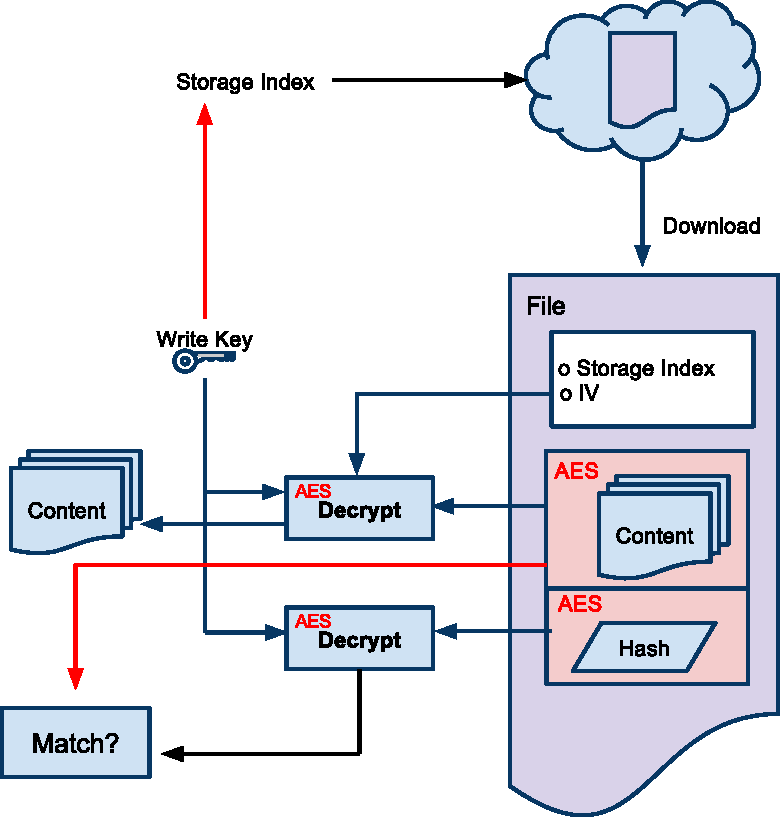
\includegraphics[width=\columnwidth]{CryptoOpenFile.pdf}
    \caption{Behind the scenes: Downloading a file}
    \label{fig:CS:OF}
\end{figure}

\subsubsection{Create Directory}

Creating and uploading a directory are illustrated in Figure \ref{fig:CS:CD}.
The process is more complex than for files, because it has to support
changing the contents of the folder.

\begin{figure}[h!]
    \centering
        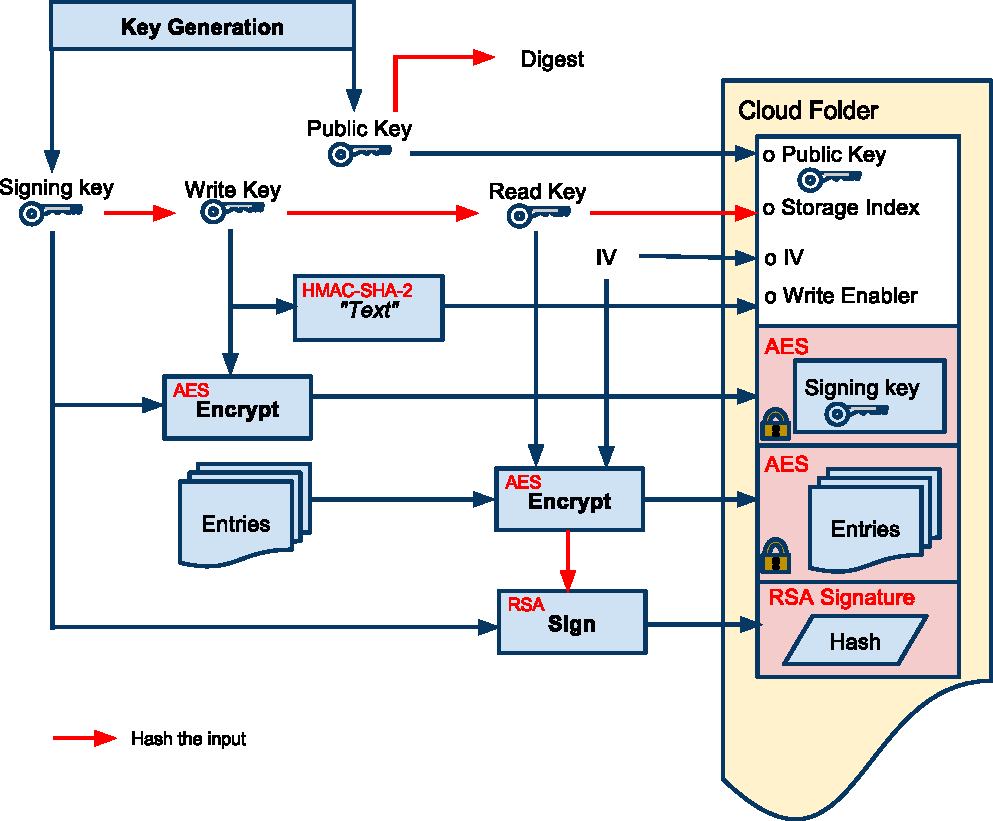
\includegraphics[width=\columnwidth]{CryptoCreateFolder.pdf}
	    \caption{Behind the scenes: Creating a directory}
    \label{fig:CS:CD}
\end{figure}

Firstly, an asymmetric key pair is generated, and forms the private
\emph{signing key} and the \emph{public key}. The signing key is hashed to form
the \emph{write key}, and again to form the \emph{read key}, and once more to
form the storage index.

The contents of the folder is encrypted with the read key and a random
\ac{IV}. The resulting ciphertext is hashed and signed with the signing
key. The signing key is further encrypted with the write key, and together with
the ciphertext, the public key, the \ac{IV} and the signature, uploaded to the
server.

The write enabler is deduced from the write key with the use of a
\ac{MAC} function and a fixed message. It is transferred alongside the
directory. The write key is stored together with a hash of the public key in
the capability.

\subsubsection{Open Directory}

Opening a directory involves both downloading, verifying and decrypting the
directory. The verification process is illustrated in Figure \ref{fig:CS:VOD}
and decryption is illustrated in Figure \ref{fig:CS:OD}.

\begin{figure}[h!]
    \centering
    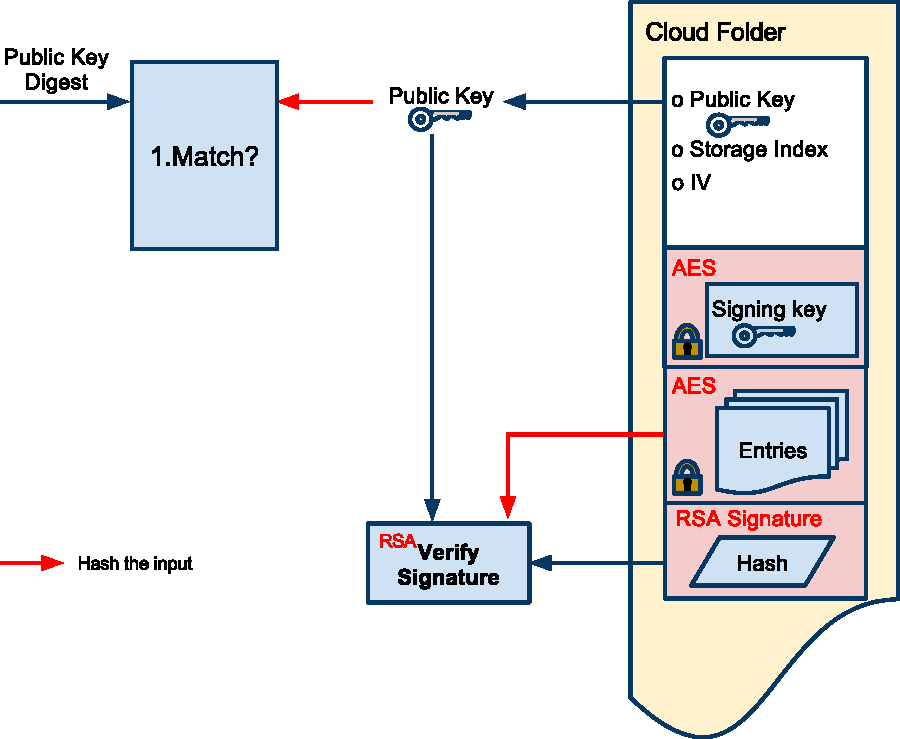
\includegraphics[width=\columnwidth]{CryptoVerifyOpenFolder.pdf}
    \caption{Verifying a directory}
    \label{fig:CS:VOD}
\end{figure}

\begin{figure}[h!]
    \centering
    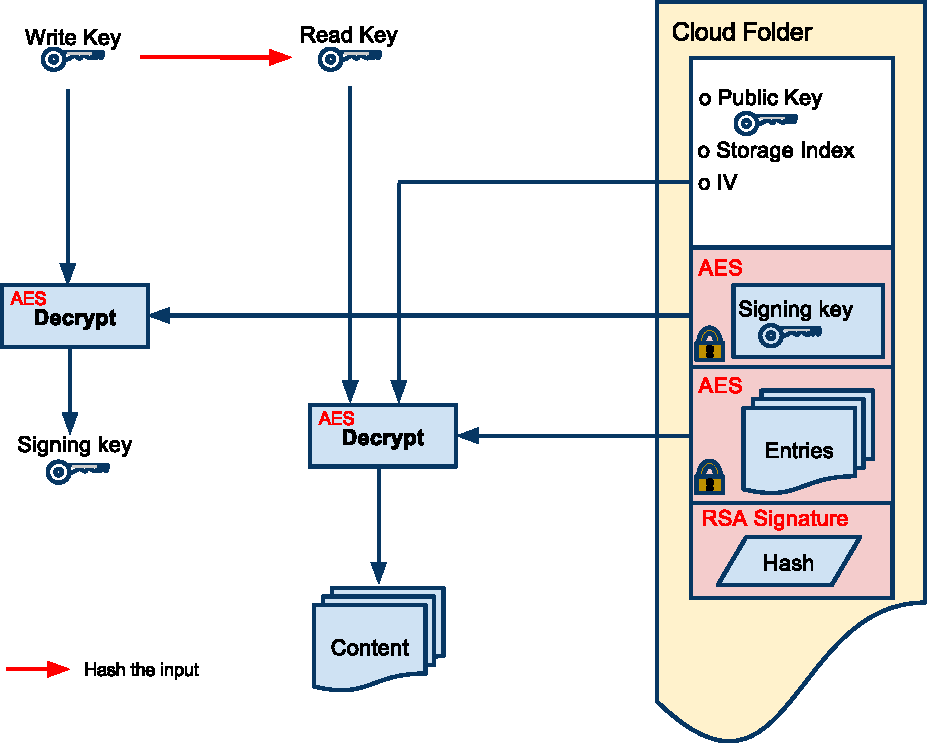
\includegraphics[width=\columnwidth]{CryptoOpenFolder.pdf}
    \caption{Decrypting the contents of a directory and obtaining the signing
    key}
    \label{fig:CS:OD}
\end{figure}

From the capability, the user obtains the read key together with the storage
index. From the server, the user receives the encrypted contents of the folder,
the \ac{IV}, the signature for the folder and the public key. The user verifies
that the public key is correct by hashing it and matching it against a hash
stored in the corresponding capability. Afterwards, the public key is used to
verify the signature. If both these checks pass, the folder is decrypted with
the read key and the \ac{IV}.

\subsubsection{Modify Directory}

In addition to read the contents of a directory, the user might want to write
to it as well. The process of doing this, is similar to initially creating the
first directory. The key difference, is that the user already has the write key
in the form of a capability, and must use this to decrypt the encrypted signing
key which resides on the server, instead of generating a new one.

A new \ac{IV} is generated, and the content of the folder is encrypted, and
signed by the signing key. The \ac{IV}, the signature and the encrypted
contents are then uploaded to the server. The write enabler is also sent
alongside, which is deduced in the same way as when creating a new folder.

\subsection{Recommendations for Cryptographic Primitives}
\label{sec:cryptoprimitivechoice}

For the proposed cryptographic scheme to be secure, it needs secure
cryptographic primitives. More specific, it needs a symmetric cipher, a
cryptographic hash function, a \ac{MAC} function, a key stretching function,
and a function for digital signatures, as observed in Figures \ref{fig:CS:CF},
\ref{fig:CS:OF}, \ref{fig:CS:CD}, \ref{fig:CS:VOD} and \ref{fig:CS:OD}.
Additionally, primitives for a secure channel between the client and the server
has to be established.

These primitives needs to be set in accordance with the security requirements
established in Section \ref{sec:criteria}. Additionally, the hard part of
selecting appropriate cryptographic primitives, is trying to predict for how
long the primitives will be secure. \citet{keylength} compares studies listing
predictions on how long primitives will be secure based on different sources
with different predictions.

\subsubsection{Symmetric Cipher}
\defcitealias{ecrypt2_2010}{ECRYPT II}

For a symmetric cipher we recommend the \ac{NIST} standard \ac{AES}, and a key
size of 128 bit should suffice. \citetalias{ecrypt2_2010} \cite{ecrypt2_2010}
has one of the more pessimistic predictions on how how secure this choice is,
saying data encrypted with a key size of 128 bit should be secure until
2030-2040.

The gain of not choosing a larger key is a somewhat greater performance --
\ac{AES}-128 uses 10 transformation rounds while \ac{AES}-256 uses 14 -- and
of course that the keys are smaller to store. However, for a new system there
are really no reason not to select a key size of 256 bit \cite{schneier}.

\paragraph{Mode of operation} The mode of operation we recommend is \ac{CBC}
for the encryption of file and folder contents. This is based more on
practical advice than on security considerations. \citet{schneier} advices the
use of either \ac{CBC} or \ac{CTR} mode, where \ac{CBC} mode is easier to
implement correctly.

For the encryption of the signing key, \ac{ECB} can be used, since the key is
encrypted exactly once and the data is considered random.

\paragraph{Padding} One negative consequence of using \ac{CBC}, is that it
requires that the plaintext is an exact multiple of the block length, i.e. 128
bit. Since this is not always the case, a padding scheme will be required. A
padding scheme does not have any security implications as long as it is
reversible \cite{schneier}, at least not for \ac{CBC}. Based on this, any
available padding scheme can be used.

\subsubsection{Cryptographic Hash Function}

The \ac{SHA}-family is the current standard for cryptographic hash functions,
and from this we recommend double \ac{SHA}-256. The cryptographic scheme
requires the hash function to have an output of at least the size of the key
used for encryption. \ac{SHA}-1 has an output of 160 bits and could have
been used for 128 bit key size, but is not recommended for use in new
systems \cite{nist_sha1}. The use of double \ac{SHA}-256 compared to single, is
to prevent a length-extension attack \cite{schneier}.

\subsubsection{Signature Algorithm}

For a signature scheme, the most commonly used algorithm seem to be either
\ac{RSA} or \ac{DSA}. Both functions would work, but we recommend \ac{RSA},
primarily because Tahoe-\ac{LAFS} made the same choice.

There might be a performance bonus in selecting \ac{RSA}. An internet
draft \cite{dsa_sha2} suggests that \ac{DSA} is about three times faster than
\ac{RSA} at signing, but \ac{RSA} is about ten times faster at verifying a
signature. A performance comparison from \citet{msdn_perf} suggest that
\ac{DSA} is 29\% faster at signing and \ac{RSA} is 29\% faster at verifying
signatures. Verification, in the form of opening a folder, is an operation we
believe most users will do significantly more than updating and creating
folders.

Multiple sources cited in \citet{keylength} recommend at least 2048 bit as the key length
used in \ac{RSA}.

\subsubsection{\ac{MAC}}

The use of the \ac{MAC} function in \ac{CSV} is somewhat special. The
definition states that a MAC function is used for authenticating messages.  As
depicted in Figure \ref{fig:CS:CD}, the output of the \ac{MAC} function is
another key. By presenting this key, a user verifies \emph{to the server} that
he is in possession of the write key for a folder and thereby authenticated and
authorized to change the folder contents. The key difference is that the
\ac{MAC} is used to verify that a user has write access, and not the contents
of the message sent.

Because of the usage of the \ac{MAC} as a simple key derivation function, the
most important factor to consider when choosing a primitive, is that it should
be infeasible to go from the result, back to the original key. On the basis of
this, \citet{schneier} recommend HMAC-SHA256.

\subsubsection{Secure Channel}

The secure channel can be provided in the form of the client and the server
communicating over \ac{TLS}. As this is a technology under continuous scrutiny,
we recommend setting the available parameters as high as possible to meet the
demands of the current situation. The reason for not specifying this more
thorough, is that libraries and software, used both server- and client-side,
may have limitations.

As an example, in the proof of concept system created, we used \ac{RSA} with a
key length of 4096 bits and \ac{SHA}-256 to create the certificate, and set the
server to only allow the strongest ciphers available.

\subsubsection{Encrypted Keyring} 
\label{sec:PBKD}

The locally stored root capability should be encrypted in some form, and a
scheme that should be compatible with most terminals is a password based key
derivation function. For this \ac{NIST} recommend \ac{PBKDF2}
\cite{pbkdf_nist}. The iteration count is to be set at high as
possible while at the same time maintaining acceptable performance, but with a
minimum of 1000. The salt should be at least 128 bit and randomly generated.
For the pseudorandom function, the recommendation is to use H\ac{MAC} with any
\ac{NIST} approved hash function.

We also looked at the usage of \ac{PBKDF2} in \ac{WPA}, and what security it
provides against brute force attacks. \ac{WPA} is used because the utilization
of \ac{PBKDF2} is similar to the one in our scheme. It uses 4096 iterations,
and H\ac{MAC}-\ac{SHA}-1 as the pseudorandom function. So far, the most
effective brute force attack against \ac{WPA} was published on Black Hat DC
2011 by a security researcher named Thomas Roth. He proved that anyone can
crack \ac{WPA} passwords with a speed of up to about 400 000 passwords per
second, using multiple Amazon \ac{EC2} cluster \ac{GPU} instances
\cite{rothwpa}. His findings also indicate that Amazon themselves can reach an
even higher unknown brute force speed. The same researcher has also hinted that
he might be able to reach 1 million keys per second with a similar setup
\cite{rothblog}.

With this in mind, we recommend at least the same amount of iterations to be
used in our scheme as in \ac{WPA}, i.e. 4096 rounds. This should yield
acceptable performance on most devices. The most elegant solution, would be to
fine tune this on a per device basis. The client can time the calculation of
4096 iterations, and increase the number if the computation is too fast. The
pseudorandom function should be H\ac{MAC}-\ac{SHA}-256, since \ac{NIST}
recommends against utilizing \ac{SHA}-1 in new applications. The salt should be
at least 128 bits.

\paragraph{Password Requirements}

\ac{NIST} also recommends that passwords should be at least 10 characters long.
If we assume that every password is alphanumeric, there exists $62^n$ different
passwords for a password of length $n$. With the stated theoretical results of
1 million passwords per second, this means that \emph{any} password of length 9
and 10 is cracked in at most 429 and 26614 years respectively. These
calculation does not take anything but the claimed current cracking speed by
Roth into account.

The results are only applicable in the real world if we can guarantee that a
user actually chooses a random password, which is probably not true. A more
realistic setting is that the attacker uses some dictionary, and that a user's
password is not strictly random. By this rationale, it is more important to be
safe than sorry, and for password guidelines we therefore recommend:

\begin{itemize}
\item Password length $>= 10$.
\item Password must include at least one capital letter, one small letter and
one number.
\end{itemize}

\section{Server Implementation}

The server, in the most basic form, has to support two operations -- sending
and receiving files. In addition, an extra layer is needed to support user
management and access control to able to allow modification of folders.
This section describes the server implementation for the proposed scheme.

\subsection{Communication and Architectural Patterns}

By definition, cloud applications are accessible over the Internet. The system
we are creating, should be able to send and receive files and information from
a server in the cloud. The \acf{HTTP} is the foundation of data communication
for the World Wide Web. The protocol is well tested, will pass through most
firewalls and has a multitude of available libraries in programming languages.
To get a working server, we can also use any existing web server as a
foundation, which will decrease total development time. Thus, \ac{HTTP} was
chosen as our communication protocol.

\subsubsection{\acs{REST}} The Web is built around an architectural style
called \ac{REST} \cite[ch. 5]{fielding}, which is defined by four interface
constraints: identification of resources, manipulation of resources through
representations, self-descriptive messages, and, hypermedia as the engine of
application state. In addition, \ac{REST} dictates five\footnote{And one
optional, Code on demand, which is not applicable for our system.}
architectural constraints \cite{fielding}. Our server application adheres to
these constraints, or \emph{patterns}, as follows:

\begin{description}
  \item[Client-server] \hfill \\
    This server will be the server part of the client-server pattern.

  \item[Stateless] \hfill \\
    Since the server is just a simple key-value file store, it does
    not need to keep state.

  \item[Cacheable] \hfill \\
    The server could easily add caching, by putting each encrypted file in
    memory as downloaded, and e.g. using the Least-Frequently Used algorithm for
    choosing which items to swap out. In addition, for every update of a folder,
    the corresponding cache item has to be marked as invalid.

  \item[Layered system] \hfill \\
    Layers are used to encapsulate, separate and hide functionality.
    Figure \ref{fig:IM:layers} illustrates the layers of the server application.

  \item[Uniform interface] \hfill \\
    The interface between clients and server(s) are given by the URI scheme in
    Table \ref{tbl:IM:restinterface}. A write enabler
    must also be provided together with the storage index when a folder is
    uploaded.
\end{description}

\begin{figure}[h!]
    \centering
    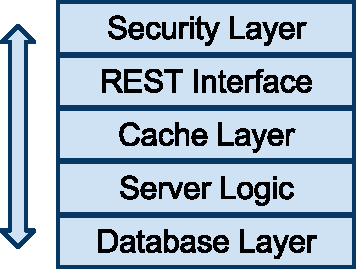
\includegraphics[scale=0.6]{ImplementationServerLayers.pdf}
    \caption{Architectural layers in the server application.}
    \label{fig:IM:layers}
\end{figure}

\begin{table}[h!]
    \centering
    \caption{The \acs{REST} interface of the server application.}
    \begin{tabular}{|l|l|}
        \hline
        \multicolumn{1}{|c}{\textbf{\acs{URI}}} & \multicolumn{1}{|c|}{\textbf{Description}} \\
        \hline
        \texttt{/put/<storage index>} & Creates or updates encrypted file \\
        \hline
        \texttt{/get/<storage index>} & Retrieves encrypted file \\
        \hline
    \end{tabular}
    \label{tbl:IM:restinterface}
\end{table}

In this context, resources are the encrypted files, and the architectural
constraints of \ac{REST} also matches that of our system as a
whole. Thus, the server application is designed in a \acs{REST}ful manner.

\subsubsection{Secure Channel} Since we are utilizing \ac{HTTP}, we can
easily add an extra layer of \ac{TLS} to form \ac{HTTPS}. This makes it more
difficult for potential attackers to intercept messages, and also provides
protection against the \ac{MITM} attacks. It also provides protection against
eavesdropping, which would have revealed the write enabler for folders and
enabling an attacker to delete folders. The top-most layer of Figure
\ref{fig:IM:layers} thus refers to \ac{TLS}.

\subsection{Environment}

The Python programming language in a Linux environment was chosen as development
platform, together with a set of applications, interfaces and micro frameworks.
The rationale for each of these follows.

\paragraph{Python} Python is a high-level general-purpose programming language.
It was chosen due to previous knowledge and experience by the
authors, in addition to its simplicity.

\paragraph{Apache} The Apache HTTP Server is a well tested and used web
server. According to \citet{netcraft}, Apache is by far the most used web server
software, and has been so since 1996. It was chosen on the basis of previous
experience and its superb documentation.

\paragraph{\acs{WSGI}} The Python \ac{WSGI} is, as the name suggests, an
interface between a web server and a Python application. It is defined in
\ac{PEP} 3333, and specifies both sides of the interface -- the
\emph{application} and the \emph{server} \cite{PEP-3333}. The server-side is
implemented in the form of an Apache module, namely \texttt{mod\_wsgi}, and the
application is where we put our code.

For each of the requests the server receives, a call
to the application function is made with two arguments -- a data structure
containing the environment variables, and a callback function for which the
application uses to return data to the requesting user via the server.

\paragraph{Pyroutes} To adhere to the \ac{DRY} principles, we chose to make use
of an open source micro framework around \ac{WSGI}, called
Pyroutes\footnote{\url{http://www.pyroutes.com/}}. It provides short cuts for the
most frequently used functionality when developing web services, as that of
\ac{URL} handling and processing of submitted user data in the form of
\texttt{GET} and \texttt{POST} requests.

Pyroutes did not, however, support the HTTP \texttt{PUT} request, so this was
implemented and contributed back to the
project\footnote{\url{https://github.com/pyroutes/pyroutes/pull/4}}.

\subsection{Implementation Details}

The code was structured as illustrated in Figure \ref{fig:IM:layout}. The file
\texttt{handler.py} provides the interface for \texttt{mod\_wsgi} and the server
application, and basically includes the \ac{URL} scheme in
\texttt{fileserver.py}. An example \ac{URL} mapping is shown in Listing
\ref{lst:IM:get}. The function \texttt{get\_file()} is registered to have the
\ac{URL} \texttt{/get} through the decorator provided by Pyroutes. After
retrieving the file from disk, a proper \ac{HTTP} response is returned,
containing required headers.

The file \texttt{filesystem.py} contains the low-level file system operations,
\texttt{save\_file()} and \texttt{retrieve\_file()}, together with a set of
helper functions to manage file access checking and database operations.  The
folder \texttt{sql/} contains \ac{SQL} code to create necessary tables in the
database, and \texttt{db.py} provides an helper function to connect to the
database.

\begin{figure}[h!]
\begin{verbatim}
|-- cloudstorage
|   |-- __init__.py
|   |-- db.py
|   |-- fileserver.py
|   |-- filesystem.py
|   |-- settings.py
|   `-- sql
|       `-- write_enablers.sql
|-- handler.py
`-- tests
    `-- filesystem_tests.py
\end{verbatim}
    \caption{Server module structure}
    \label{fig:IM:layout}
\end{figure}

\lstinputlisting[language=Python,breaklines=false,label=lst:IM:get, caption=URL mapping in fileserver.py]
{listings/fileserver.py}

\subsubsection{Authorization functionality}

The only functionality of the authorization layer implemented, is the
server-side verification that a client has proper access to overwrite a folder,
e.g. when a client wishes to update a folder with new contents.

When a client first uploads a new folder, it provides a write enabler,
which the server adds to the database along with the storage index of
the folder. For every subsequent request to write to this folder, the server
verifies that the provided write enabler is equal to that in the database.

If a client tries to put a folder with a storage index that already exists, the
server replies with an error code if the client in addition does not provide
the correct write enabler.

\section{Client Implementation - Android}

The proof of concept client we have implemented, is made for devices using the
Android operating system, which is based on Linux. The \ac{SDK} for making
Android applications, is essentially a somewhat modified version of Java.

Most devices that use the Android operating system are mobile phones or
tablets, which implies that they are more limited in terms of computational
power and memory, compared to a modern computer. The point of making
the client for such a device, i.e. a \emph{smart phone}, is the growing
availability, and the flexibility these devices provide. A user carries the
device everywhere, it provides network connectivity, and is almost always on.

A nice side effect of developing on a smart phone platform, is that if the
software performs well on a constrained device, it will almost certainly
perform just as well on any faster device.

\subsection{Environment}

The client was made on the Android platform and written in the Java programming
language, together with a set of frameworks. The rationale for these are as
follows.

\paragraph{Android} The Android operating system is made by Google, and is most
commonly found on mobile phones and tablets. The platform choice of Android was
done based on hardware availability and familiarity with developing on the
platform and the programming language.

\paragraph{Java} Java is a high-level, object-oriented programming language.
Applications written in Java runs in a \ac{JVM}, which implies that a Java
application can run on almost any device which has a \ac{JVM}.

The ``\ac{JVM}'' on Android is called \emph{Dalvik}, but it is strictly not a
\acl{JVM} as the bytecode on which it operates is not Java bytecode.
After the regular Java compiler has created the \texttt{.class} files, a Dalvik
tool transforms them to another class file format called \texttt{.dex}
\cite{dalvik}.

\paragraph{HttpComponents} Apache HttpComponents are a set of libraries for
\ac{HTTP} transport in Java. The part used in our client is called HttpClient.
Android incorporates parts of this client in its runtime environment. The use
of this library adheres to the \ac{DRY} principles as defined in Section
\ref{methodology}.

\paragraph{\ac{JCA}} \ac{JCA} is an architecture for doing cryptographic
operations in Java. The architecture is based on principles of implementation
independence, implementation interoperability and algorithm extensibility.
Basically what this means, is that each \ac{JVM} can have different
implementations of the cryptographic primitives, but the developer does not
necessarily need to know which ones are available.

\paragraph{ZXing Barcode Scanner} ZXing Barcode Scanner\footnote
{\url{http://code.google.com/p/zxing/}} is a popular Android application which
can be used by other Android applications to both scan and generate barcodes.
By the use of this application, we adhere to the \ac{DRY} principles by not
creating our own code to generate barcodes.

\subsection{Architectural Patterns}

\paragraph{Client-Server} The client we have implemented is the client part of
the overall client-server pattern of the system.

\paragraph{Pipe-and-Filter} The basis of the pipe-and-filter pattern is that
there exist a chain of processing elements, where the output of one element is
the input of the next element. We use this for file uploads and downloads to
limit the memory usage of the client, as well as to increase performance.

\paragraph{Asynchronous Pattern} We use asynchronous calls to slow operations
-- e.g. file upload and key generation -- extensively, to prevent the user
interface from hanging and to deliver a smoother user experience in general.

\subsection{Implementation Details}
\label{sec:cli:impl:det}

The following section describes the code structure of the client
implementation, in addition to cryptographic entities used.

\subsubsection{Structure}
The source of our client is logically separated into two entities --
\texttt{CSVlib} and \texttt{CSVAndroid}. \texttt{CSVlib} is a pure Java library which
contain the necessary entities, cryptographic operations and communication
calls required for the client. \texttt{CSVAndroid} contains primarily a graphical user
interface to make use of \texttt{CSVlib} on an Android device.

\subsubsection{Cryptographic Entities}
\label{sec:cryptoentities}

All the cryptographic entities -- namely folders, files and capabilities -- are
all part of \texttt{CSVlib}. Their relationship can be seen in Figure
\ref{fig:CSVlib:overview}.

\begin{figure}[h!]
    \centering
    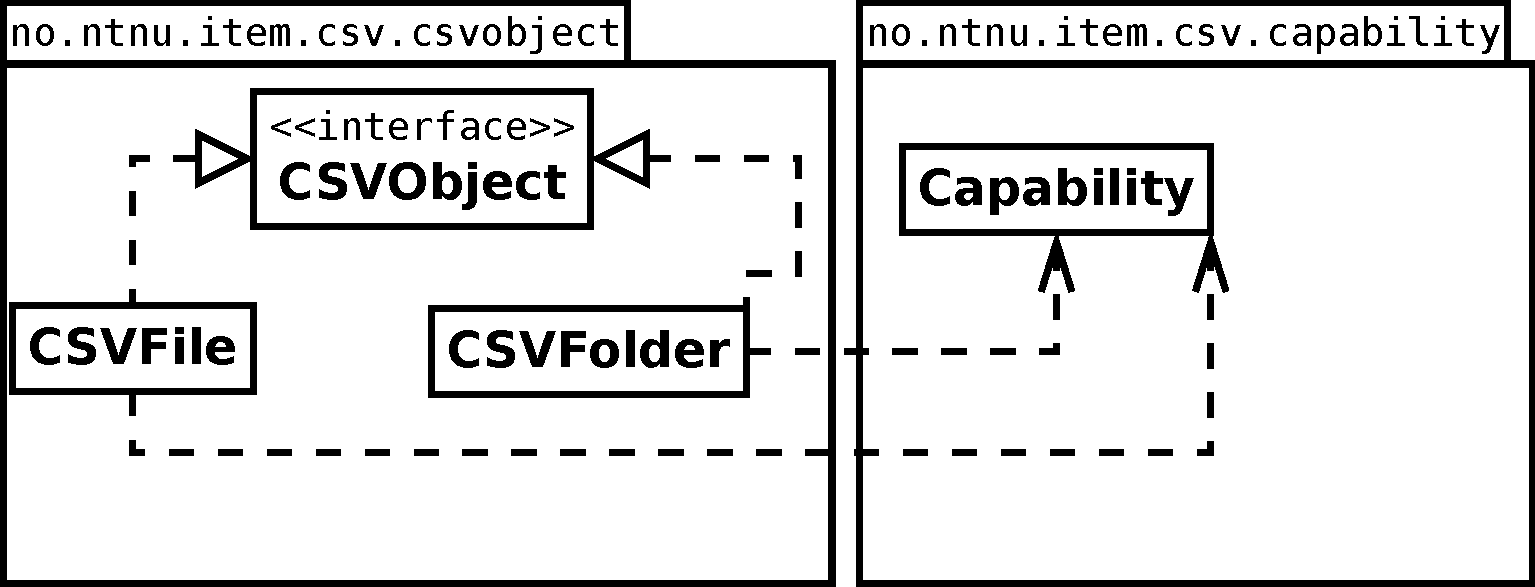
\includegraphics[scale=0.4]{csvobjects.pdf}
    \caption{Cryptographic entities and their relations}
    \label{fig:CSVlib:overview}
\end{figure}

\paragraph{Capabilities} Capabilities are containers for cryptographic keys and
information to identify a corresponding object. They will will contain
information to identify an object as either a file or a folder, and have the
information to read, write and verify that object.

Capabilities are stored server-side in folders in its serialized form shown
in Figure \ref{fig:CAP:serial}. \emph{Object Type} specifies if the capability
represents a file or a directory, with values \emph{F} or \emph{D}
respectively.

\begin{figure}[h!]
    \centering
    
\includegraphics[scale=0.6]{CapabilitySerialization.pdf}
    \caption{Serialized form of a capability}
    \label{fig:CAP:serial}
\end{figure}

\emph{Key Type} specifies the permissions the key will grant on the object, and
can be either \emph{RO} (Read-only) or \emph{RW} (Read-write).

The different parts are separated by the colon character. The key and verify
strings are encoded in Base32 \cite{rfc4648}, which means that the 128 bits
these strings are represented by, will be replaced by an alphabet of 32
different symbols, namely A-Z and 2-7. This makes it possible to read for a
human with few mistakes or misunderstandings.

\paragraph{Folders}

A folder is represented by the class \texttt{CSVFolder}. A \texttt{CSVFolder}
object is a collection of aliases and their corresponding capabilities. For the
most part, the data stored in a folder is so small that it can easily live for
as long as needed in the memory of the client.

When a folder is created or updated, the content is serialized and encrypted,
before it is uploaded to the server directly from memory. The serialization for
each item in a folder is on the form \textbf{alias;capability}, where the
capability itself is also serialized.

\paragraph{Files}

A file is represented by the class \texttt{CSVFile}. While a folder in general
is small, a file can be of any size, even larger than the \ac{RAM} on the
device.

To keep the memory footprint low, we use the pipe-and-filter architectural
pattern to stream data all the way from the server to the device, or vice
versa, through encryption and verification.

An example of how we do this for uploads, is shown in Listing
\ref{lst:inputstream}.

\lstinputlisting[label=lst:inputstream, caption=Pipe and filter upload of a file]
{listings/fileupload_example.java}

The \texttt{InputStreams} are chained together, with the effect that a read
from \texttt{readBuffer} will trigger a read trough the whole pipe. The
\texttt{DigestInputStream} will update the state of the hash function, but is
transparent in the sense that what goes into the stream will also be what comes
out. The \texttt{CipherInputStream} on the other hand, will output an encrypted
stream of the data from the file. To handle different input/output speeds,
buffers are placed between each step of the stream to gain some performance.

\subsubsection{Communication with Server}
% Do not repeat what is said in Server equivalent section
% Apache commons, Serialization of objects

For \ac{HTTP} transport, we utilize the Apache Software Foundations
HttpComponents Client\footnote{ \url http://hc.apache.org/}, also known as
HttpClient. This Client offers support for authenticated requests to a server, and both
upload and download through \texttt{PUT} and \texttt{GET} requests
respectively.

We wrap communication with the server in two classes,
\texttt{Communication.java} and \texttt{CSVFileManager.java}.
\texttt{Communication.java} provides functionality for sending and retrieving
data from our server, while \texttt{CSVFileManager.java} provides specific
methods for sending and receiving the encrypted objects, \texttt{CSVFile} and
\texttt{CSVFolder}.

\subsubsection{Deviations in the Choice of Cryptographic Primitives}
\label{sec:client:deviations}

The implementation of the proof of concept client deviates from the
recommendation given in Section \ref{sec:cryptoprimitivechoice}.  This occurred
as a result of new discoveries that were made while analysing the system. All
unfortunate deviations are corrected with a patch file submitted along with the
code attachment, described in Appendix \ref{ap:attachments}. For the other
primitives we follow the recommendation.

\paragraph{RSA Key Length} The key length chosen for the RSA cipher is 1024
bits, in contrast to the argued 2048 bits. It is therefore important to notice
that all measurements, presented in Chapter \ref{ch:experimental} and
\ref{ch:results}, are based on an RSA key length of 1024 bits.

\paragraph{AES Key Length} The key length used in our implementation is 128 bit
for \ac{AES}. The reason to prefer a shorter key length in \ac{CSV} is to make
manual key exchange less cumbersome. 256 bits are however preferred.

\subsection{Sharing}

A \emph{shared folder} is a folder which two or more people have the required
capability for.

The problem of creating a share with someone, is that you have to verify that
you are actually sharing with the correct person. The data, or \emph{secret},
that will have to be shared, is a serialized form of the capability of the
shared folder, as shown in Figure \ref{fig:CAP:serial}.

The client supports two methods of doing this. The most cumbersome is having to
manually copy the key from one user's client to another, and afterwards verify
that the key for the selected folder is correct. An example of this can be seen
in Figure \ref{fig:CSVAndroid:manualimport}. This feature is also needed to
support out-of-band methods for establishing a share, e.g. through the use of
\ac{PGP}.

\begin{figure}[h!]
    \centering
    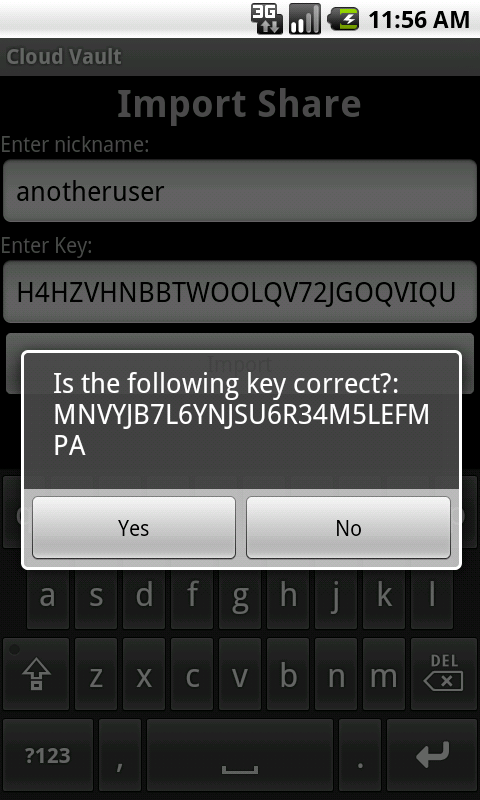
\includegraphics[scale=0.4]{client-manualimport.png}
    \caption{Establishing a share by copying the key}
    \label{fig:CSVAndroid:manualimport}
\end{figure}

The other possibility is to make use of a \emph{\ac{QR} code}, which is a
matrix barcode that can store information. This means that one user will
generate a barcode, and the other user can scan that code using
the camera on his device. Figure \ref{fig:CSVAndroid:barcode} illustrates how
this code will look. The barcode contains both the key and the verification for
the shared folder. Once two users have shared a folder once, that folder can be
used for all future shares, which means that the two people will never have to
meet and do the capability exchange again. The identity has thus been verified.

\begin{figure}[h!]
    \centering
    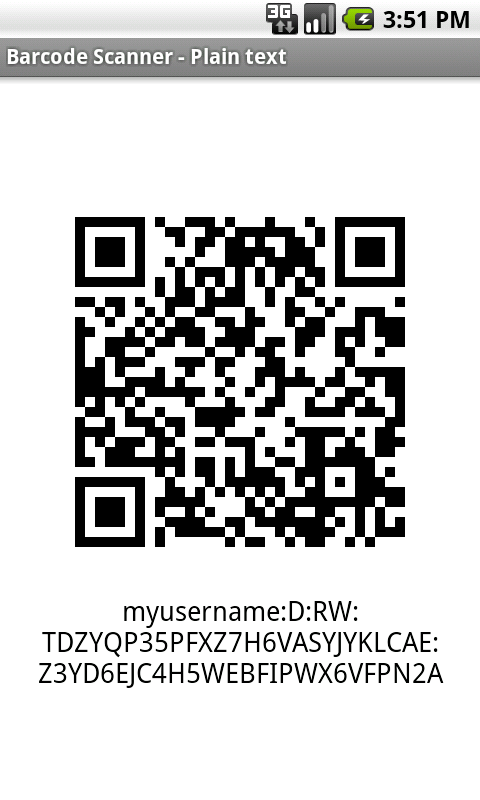
\includegraphics[scale=0.4]{client-barcode.png}
    \caption{Establishing a share by using barcodes}
    \label{fig:CSVAndroid:barcode}
\end{figure}

\subsection{Adding a New Client}

Using more clients, or different devices, is almost the exact same as sharing,
and is solved in the same manner. The only difference is that the capability
that needs to be transferred, is that of the root folder. It is also possible
to take any other folder and use as a new root for the new client if that is
the wish of the user.

\subsection{Securing the Client}

For a user to access her root folder, the client will have to know the
capability of that folder. This is clearly too much random data for most users
to remember, so the capability will have to be stored on the client.  The
client might be stolen or broken into by some means, and if the capability is
stored in clear text, it is easily compromised. We therefore implement a
locally stored encrypted keyring which contains this capability.

\ac{PBKDF2} is used with 4096 iterations and H\ac{MAC}-\ac{SHA}-256, together
with a user defined password to derive a 128 bit encryption key. The keyring is
then encrypted with \ac{AES} and the derived key, in \ac{ECB} mode.
Figure \ref{fig:KeyringFormat} illustrates the keyring contents. The username,
password, scheme, hostname and port fields are used to remember the credentials
needed to get access to the server.

\begin{figure}[h!]
    \centering
    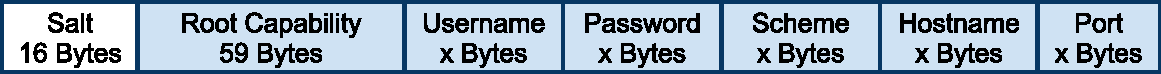
\includegraphics[scale=0.6]{KeyringFormat.pdf}
    \caption{The keyring format with encrypted fields shaded in blue}
    \label{fig:KeyringFormat}
\end{figure}

\subsection{User Interface}

We have tried to make a user interface that is easily understandable by a
novice user, both in terms of \emph{where to click} and in terms of how we name
cryptographic operations. For instance we never use the word \emph{capability}
in the client. To make the \ac{GUI} even easier to understand, we have created
a video that examines the most important user interactions with the
application. The video is available in the attachment, which is further
described in Appendix \ref{ap:attachments}.

In addition to the attached video, this section will present the most important
parts of the implemented \ac{GUI}. 

\paragraph{Main Screen}

The main screen of the application is shown in Figure
\ref{fig:CSVAndroid:mainscreen}. Before the user gets to this screen, she will
have to unlock her encrypted keyring with her password. If it is the first time
the application is started, she have to enter her online credentials, and get a
choice to either import an existing root folder, or to generate a new one. In
both cases, the user will have to choose a password to encrypt the root
capability. The most common action from the main screen would be to
\emph{Browse the Vault} -- in other words to explore the available files stored
on the server.

\begin{figure}[h!]
    \centering
    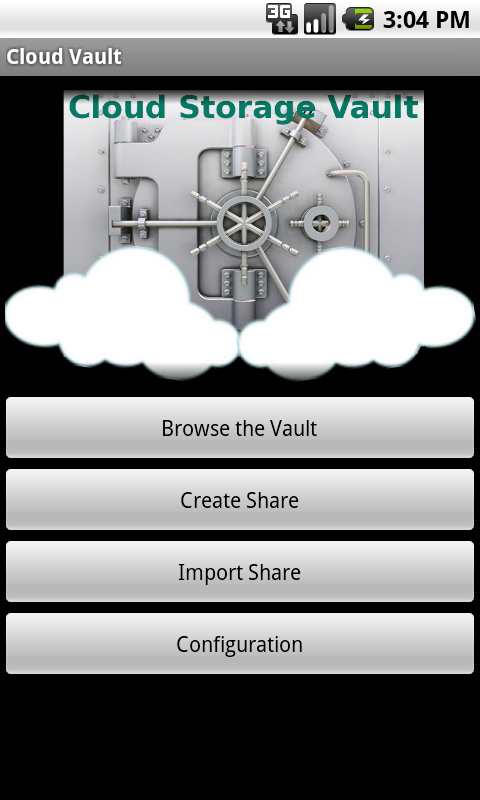
\includegraphics[scale=0.4]{client-mainscreen.png}
    \caption{Main screen of the client application}
    \label{fig:CSVAndroid:mainscreen}
\end{figure}

\paragraph{Browse the Vault}

The interface for browsing files stored in the cloud, is made in what we
understand as a common and understandable way of interpreting users actions on
the Android platform, and can be seen in Figure
\ref{fig:CSVAndroid:remotebrowse}. Tapping a file will download that file, and
tapping a folder will open that folder.

\begin{figure}[h!]
    \centering
    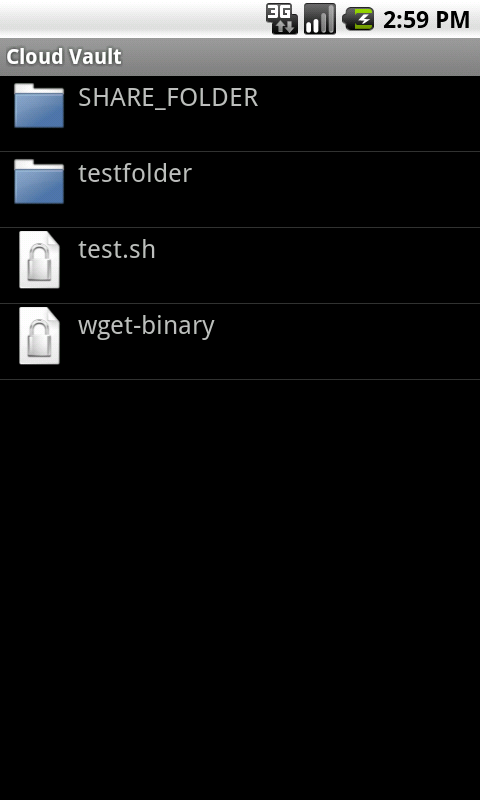
\includegraphics[scale=0.4]{client-remotebrowse.png}
    \caption{Browsing the cloud storage from the client}
    \label{fig:CSVAndroid:remotebrowse}
\end{figure}

Selecting files to upload is treated in a similar way. To reveal this option,
the user have to press the \emph{Menu}-button. The user will then be allowed to
browse her local file system for the file she wishes to upload, and tapping that
file will start the upload.

A long press on a file, or a folder item, will reveal the context menu shown in
Figure \ref{fig:CSVAndroid:remotecontext}. The least understandable action is
probably \emph{Unlink}, which will remove a file or a folder from the parent
folder.  The reason why it says unlink and not delete, is that the architecture
does not specify a way for deleting files. The implementation does not make
this choice either. This is further discussed in Section
\ref{sec:deletion_of_files}.

\begin{figure}[h!]
    \centering
    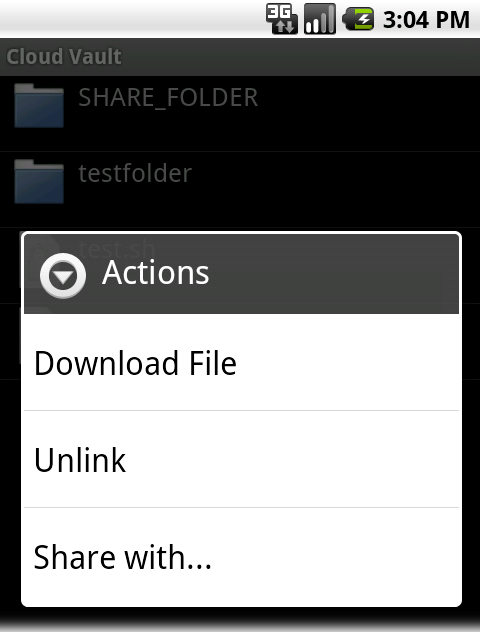
\includegraphics[scale=0.4]{client-browsecontext.png}
    \caption{Context menu showing actions available for items stored}
    \label{fig:CSVAndroid:remotecontext}
\end{figure}

%**************************************%
\chapter{Experimental Procedure}
\label{ch:experimental}
%**************************************%

This chapter describes the experimentation performed on the implemented system.
It will start by explaining the measurements on the performance of the
application. Finally, the chapter will go through the experimental procedures
taken to measure the security of the locally encrypted keyring.

\section{Performance of the Client}

We have tested the Android client on two Android smartphones, an HTC Desire and
an HTC Hero. We have also tested the Java libraries on a desktop computer. The
specifications for HTC Desire can be seen in Table \ref{tbl:device:desire}, for
HTC Hero in Table \ref{tbl:device:hero}, and the desktop computer in Table
\ref{tab:hwbf}. The server has identical specifications as the computer. We
emphasize that the measurements are meant to be taken as indications of the
performance of the scheme and implementation, and not as exact measurements.
The server was never considered as a possible bottleneck for the system, due to
all heavy operations being performed client-side.

\begin{table}
  \centering
  \caption{HTC Desire Specifications}
  \begin{tabular}{ | l | l |}
    \hline
    Name    & HTC Desire                        \\ \hline
    CPU     & Qualcomm Snapdragon QSD8250, 1 GHz \\ \hline
    Memory  & 576 MB \ac{RAM}                   \\ \hline
    Storage & Samsung Micro SDHC Class 2, 4 GB  \\ \hline
    System  & Android 2.2, Linux 2.6.32.15      \\ \hline
  \end{tabular}
  \label{tbl:device:desire}
\end{table}

\begin{table}
  \centering
  \caption{HTC Hero Specifications}
  \begin{tabular}{ | l | l |}
    \hline
    Name    & HTC Hero                          \\ \hline
    CPU     & Qualcomm MSM7200A, 528 MHz        \\ \hline
    Memory  & 288 MB \ac{RAM}                   \\ \hline
    Storage & Micro SDHC Class 6, 4 GB          \\ \hline
    \ac{OS} & Android 2.2, Linux 2.6.29.6      \\ \hline
  \end{tabular}
  \label{tbl:device:hero}
\end{table}

\begin{table}[!h]
    \centering
    \caption{Test computer Specifications}
    \label{tab:hwbf}
    \begin{tabular}{| l | l |}
	\hline
	Product		        &HP Compaq 8100 Elite SFF PC \\
	\hline
	CPU		            &Intel(R) Core(TM) i7 CPU 860 @ 2.80GHz\\
	\hline
	Memory	            &4GB \ac{RAM}\\
	\hline
    Storage             &Hitachi HDS72105 SATA2 \\
	\hline
    OS		            &Ubuntu 10.10 64 bit\\
	\hline
	Kernel Version	    &Linux 2.6.35\\
	\hline
    Network             &1Gbit wired Ethernet \\
    \hline
    \end{tabular}
\end{table}


\subsection{Measured Operations}

The construction used to encrypt, hash and transfer \emph{files}, is a pipeline
as described in Section \ref{sec:cryptoentities}. The interesting thing to
measure, is the overall speed of the pipeline, compared to a simple file
transfer with no extra operations such as hashing and encryption. To try
to pinpoint the exact bottlenecks in the pipeline, we also measure the
bandwidth we get from each of the isolated operations in the pipeline on one of
the Android devices, the HTC Desire.

\emph{Folders} are relatively small in size, and the implementation does not
include the use of a pipeline. All cryptographic operations are completed for
the whole folder prior to sending any data. The speed of these operations are
therefore measured and includes the following:

\begin{enumerate}
    \item The average time it takes to create a folder, i.e. initial key
        generation
    \item The time it takes to encrypt and sign a folder, with varying amount
        of data
    \item The time it takes to verify a newly downloaded folder, with varying
        amount of data
    \item The time it takes to serialize a folder, with varying amount of data
\end{enumerate}

\subsection{The Measurement Procedure}

To test the bandwidth of the pipeline for files, we measure the incoming
traffic to our server using the tool \texttt{nload}\footnote{
\url{http://www.roland-riegel.de/nload/}} during a file upload.

The average bandwidth are observed for a few seconds after the file upload has
been started, until the file upload is nearly complete. This does not take
overhead into consideration, such as the initial key generation, but for any
file with a certain size, this overhead should be neglectable.

To be able to test the different folder operations in the program code, we use
the Java function \texttt{System.currentTimeMillis()}, which we call before and
after an operation, and calculate the difference to get the time spent. When we
test operations that are dependant on the contents of a folder, we do this with
each containing item being 86 bytes.

\subsection{Eliminating Bottlenecks on Android Devices}

On the Android devices, three possible bottlenecks that we might be able to
control are identified: the \emph{network}, the \emph{memory card} and our
implementation of the \emph{application}.

The mobile phones will normally obtain their network connection through a
wireless protocol that varies naturally in throughput, e.g. \ac{UMTS}. These
protocols work just fine, but from a measurement standpoint, we want to have a
fast and stable connection. The solution was therefore to connect the Android
devices to the test computer, and use the computers network through the
\ac{USB} interface.

Another bottleneck, might be the memory card. The \emph{class} of a memory card
will identify the least sustained write speeds obtainable from the card in a
fragmented state \cite{sdcard}. The class number $X$ represents this guarantee
in $X$ MB, so a Class 2 card guarantees a speed of 2 MB/s. However, there are
the possibility that the card can perform significantly better than what the
class number indicates.

\subsection{Sources of Error}

The trouble with measuring performance on operations that are relatively quick,
is that they are vulnerable to \emph{noise} from the system. The Android
system comes with a lot of built-in services that runs sporadically, and hence
affect the measurements. However, the small and quick operations are not
necessarily fascinating to measure -- the interesting behaviour to observe is
how their performance is affected when the amount of data is increased. The
goal of the client is to deliver a quick and smooth experience for the user.

We cannot explicitly tell what the speed of either the network nor the memory
card are, and this is thus another error source. But by comparing the speed for
file operations in \ac{CSV} with the modified version without encryption and
hashing, we should get an indication about how quick the software can be.

\section{Security of the Encrypted Keyring}
\label{sec:BFLK}

The locally stored and encrypted keyring can be considered a security risk if
it somehow ends up in the hands of an attacker, either by a device being lost
or by an intrusion in to a device. Even though the keyring is encrypted, it
might be prone to brute force or dictionary attacks. If an attacker is able to
decrypt the keyring, enough information to access the root folder of a user is
obtained, and thus all the files stored by the user as well.

When considering brute force attacks, it must be emphasized that it is the
user's password, indirectly encrypting the keyring, that is the target
weakness. A brute force attack on the 128-bit \ac{AES} encryption key directly
will be inefficient as it involves a key space of $2^{128}$ keys. The
possibility of dictionary attacks would additionally disappear, as the
encryption key is generated in a pseudorandom manner. This section describes
our approach to attack the keyring.

\subsubsection{Keyring Format}

The format of the encrypted keyring is given in Figure \ref{fig:KeyringFormat}.
It is encrypted with 128-bit \ac{AES} in \ac{ECB} mode, but the key is not
randomly generated. The key is given by the key strengthening function
\ac{PBKDF2}, but this is based on a password set by the user, which is why this
key is potentially weaker than the keys for files and folders.

An attacker will also know some of the plaintext of the keyring. The
serialization of a capability for a writeable folder will start with
\textbf{D:RW:}, followed by 16-byte of Base32-encoded data, another colon
(\textbf{:}) and then 16 more bytes of Base32-encoded data. In addition, the
fields in the decrypted form of the keyring are separated by the pipe character
(\texttt{|}).

\subsubsection{General Procedure}

To perform a brute force or dictionary attack on the encrypted keyring, one
must decrypt the keyring for each password guessed. The decryption involves
both key derivation with \ac{PBKDF2}, and decryption with 128-bit \ac{AES} in
\ac{ECB} mode. \ac{PBKDF2} is a function that can be used with a varying number
of iterations, with the purpose of having a customizable way for users to
increase key strength. The attacks are tested on 500, 1000, 2000, 4000 and 8000
iterations.

\subsubsection{Implemented Attacks}

We created two programs designed to crack the keyring password. The first
program, named \acf{BFDA}, was designed for a single computer, while the second
program, named \acf{CDA}, was created to perform attacks by a cluster of
cooperating computers.

Both use dictionary attacks, but \ac{BFDA} is also capable of a plain brute
force attack. The source code and compiled \texttt{.jar} files for both
programs can be found in the attached disc. Implementation details are given in
Appendix \ref{ap:other}.

\subsubsection{Configuration}

\ac{BFDA} requires Java with the \ac{JCE} and Jurisdiction Policy files which
enables Java to use stronger cryptographic primitives. It also depends on Java
being configured to use Bouncy Castle as its primary \ac{JCE} provider. These
prerequisites are required because the keyring is encrypted using Bouncy
Castle, as this is used by default on the Android platform.

\ac{CDA} requires almost the same configuration as \ac{BFDA}, but naturally for
each node in the cluster. Additionally, the cluster must be configured with
Apache Hadoop.

The steps we performed to set up Java with Bouncy Castle and the Jurisdiction
Policy files, are as described by \citet{jce+bc}, and the guide we used for
configuring Apache Hadoop in a Cluster using Ubuntu Server, are made by
\citet{cluster}.

\subsubsection{Hardware Specifications}

The hardware specifications for the computer running \acl{BFDA} are given in
Table \ref{tab:hwbf}. The \acl{CDA} was executed over a cluster of Amazon
\ac{EC2} instances, of type \emph{High-CPU Extra Large Instances}. The hardware
specification for a single instance, used in the cluster attack, is given in
Table \ref{tab:hwcda}.

\begin{table}[!h]
    \centering
    \caption{Hardware Specifications for Cluster Instances}
    \label{tab:hwcda}
    \begin{tabular}{| l | l |}
	\hline
	Instance Type       &High-CPU Extra Large Instance\\
	\hline
	CPU		            &Intel(R) Xeon(R) CPU E5410 @ 2.33GHz\\
	\hline
	CPU Architecture    &x86\_64\\
	\hline
	RAM		            &7GiB\\
	\hline
	OS		            &Ubuntu 10.10 (Maverick Meerkat)\\
	\hline
	Kernel Version	    &2.6.35-24-virtual\\
	\hline
	I/O Performance	    &High (as defined by Amazon)\\
	\hline
    \end{tabular}
\end{table}


\subsubsection{Running \ac{BFDA}}

The command used for executing a brute force attack with \ac{BFDA} can be
seen in Listing \ref{lst:bf}. The command for running a local dictionary attack
is seen in Listing \ref{lst:da}.

\lstset{label=lst:bf, caption=Running local brute force attack}
\begin{lstlisting}
$ java -jar BFDA.jar /path/to/keyring  \
    maximum_password_length number_of_threads
\end{lstlisting}

\clearpage
\lstset{label=lst:da, caption=Running local dictionary attack}
\begin{lstlisting}
$ java -jar BFDA.jar /path/to/keyring \
    /path/to/dictionary number_of_threads
\end{lstlisting}

\subsubsection{Cloud Dictionary Attack}

\ac{CDA} was executed on 20 of the previously specified Amazon EC2 nodes. One
instance was configured as both a Hadoop \emph{master} and \emph{slave} node,
while the 19 other instances were configured as slaves.  This was done to
utilize as much as possible out of the available nodes, as the master node
performs less computational work than the slave nodes.

Multiple scripts are needed to initiate the distributed attack.
The commands executed to start the Hadoop master and slaves, and mount up the
shared, distributed file system \ac{HDFS}, are shown in Listing
\ref{lst:hadoop}. The final command enables the Hadoop cluster to support
\emph{MapReduce}. This is necessary as the \ac{CDA} attack is implemented as a
map-reduce problem. Details about Apache Hadoop, MapReduce and the
implementation of \ac{CDA}, are given in Appendix \ref{ap:other}.

\lstset{language=bash, label=lst:hadoop, caption=Starting Hadoop Cluster with HDFS}
\begin{lstlisting}
# Start HDFS and initialize master and slave nodes
$ /path/to/Hadoop/bin/start-dfs.sh

# Start a MapReduce cluster from the master node
$ /path/to/Hadoop/bin/start-mapred.sh
\end{lstlisting}

The last requirement, before executing the attack, is to copy the
desired dictionary file and keyring into the \ac{HDFS}. Copying files from the
master node to the \ac{HDFS} is done with the command shown in Listing
\ref{lst:cpHDFS}. The attack can then be started on the master node with the
command shown in Listing \ref{lst:CDA}.

\lstset{language=bash, label=lst:cpHDFS, caption=Copying files into HDFS}
\begin{lstlisting}
$ /path/to/Hadoop/bin/hadoop dfs -put /path/to/file \
    /path/to/file/in/HDFS
\end{lstlisting}

\lstset{language=bash, label=lst:CDA, caption=Executing the CDA Attack}
\begin{lstlisting}
$ /path/to/Hadoop/bin/hadoop jar /path/to/CDA.jar \
    /HDFSpath/to/dictionary /HDFSpath/to/output/file \
    /HDFSpath/to/keyring number_of_slaves \
    number_of_threads_per_slave
\end{lstlisting}

%**************************************%
\chapter{Results}
\label{ch:results}
%**************************************%

In this chapter we present the quantifiable numbers retrieved when doing the
experimentation described in Chapter \ref{ch:experimental}. This includes
performance measurements of the implemented client, and results of the attacks
performed on the encrypted keyring.

\section{Performance of the Client}

This section presents the numbers obtained from benchmarking the client, and
highlights the most important results. As mentioned in Section
\ref{sec:client:deviations} we implemented the \ac{CSV} client with a key
length of 128 bits for \ac{AES} and 1024 bits for \ac{RSA}. The results
presented in this chapter are based on this first client.

\subsection{Files}

This section shows the network speed obtained when uploading and downloading
files. Table \ref{tbl:files:encrypted} displays the obtained bandwidth when
using the \emph{unmodified} client, while Table \ref{tbl:files:unencrypted}
shows the obtained bandwidth when using the same client, but with
\emph{encryption and hashing disabled}. Table \ref{tbl:desire:pinpoint} shows
the speed of the individual, isolated operations in the process pipeline on the
HTC Desire.

\begin{table}
  \centering
  \caption{File upload on CSV}
  \begin{tabular}{ | l | r | r |}
    \hline
    \textbf{Model}    &   \textbf{Upload}  &   \textbf{Download}   \\ \hline
    Desire   &   715 kB/s & 1,25 MB/s   \\ \hline                
    Hero     &   209 kB/s & 486 kB/s    \\ \hline 
    Computer &  27,7 MB/s & 24,9 MB/s \\ \hline
  \end{tabular}
  \label{tbl:files:encrypted}
\end{table}

\begin{table}
  \centering
  \caption{File upload/download on CSV with encryption and hashing disabled}
  \begin{tabular}{ | l | r | r |}
    \hline
    \textbf{Model}    &   \textbf{Upload}  &   \textbf{Download}   \\ \hline
    Desire & 2,62 MB/s & 2,3 MB/s \\ \hline
    Hero & 1,68 MB & 1,75 MB \\ \hline
    Computer & $\sim$70 MB/s & $\sim$70 MB/s \\ \hline
  \end{tabular}
  \label{tbl:files:unencrypted}
\end{table}

\begin{table}
  \centering
  \caption{Speed of individual operations on HTC Desire with a 4,38 MB file}
  \begin{tabular}{ | l | r | r |}
    \hline
   \textbf{Operation} & \textbf{Time} & \textbf{Bandwidth} \\ \hline
   Read file to memory  & 1,141s & 3.84 MB/s       \\ \hline
   Encrypt file data    & 3,761s & 1,16 MB/s    \\  \hline
   Decrypt file data    & 3,140s & 1,40 MB/s    \\ \hline
   Hash data            & 0,358s & 12.25 MB/s   \\ \hline
  \end{tabular}
  \label{tbl:desire:pinpoint}
\end{table}


We observe that the performance of the Android devices for uploads is severely
lower for uploads than for downloads, and that this is not the case for the
computer client. We also notice that the speed with encryption and hashing
disabled, is severely higher for all three devices. From the individual results
of the HTC Desire, we identify that the encryption and decryption is the most
time consuming operation.

\subsection{Folders}

Table \ref{tbl:folder:createblank} shows the average time it takes to create an
empty folder on the different devices. Table \ref{tbl:folder:serializefolder}
exhibits figures on serialization of folders and Table
\ref{tbl:folder:encryptsign} shows the time it takes to encrypt and sign the
folder, and is visualized in Figure \ref{fig:results:signencrypt}. These three
actions are what has to be performed every time a folder is changed, while the
operation of creating a blank folder is added if the content should be added to
a new folder. Table \ref{tbl:folder:verify} displays the time the devices used
to verify an existing folder, a step which is taken by the client every time a
folder is opened. Results noted as \emph{N/A} for the HTC Hero, are operations
that lead to an \emph{Out of Memory} exception during execution.

\begin{table}
  \centering
  \caption{Create a blank folder}
  \begin{tabular}{ | l | r | r |}
    \hline
   \textbf{Computer} & \textbf{HTC Desire} & \textbf{HTC Hero} \\ \hline
    81ms  &1330ms     &2060ms    \\ \hline
  \end{tabular}
  \label{tbl:folder:createblank}
\end{table}

\begin{table}
  \centering
  \caption{Serialize the contents of a folder, with n*86 bytes of data. Time in
  ms}
  \begin{tabular}{ | l | l | l | l |}
    \hline
    \textbf{n*86 bytes} & \textbf{Computer} & \textbf{HTC Desire} & \textbf{HTC Hero} \\ \hline
    500     &   &   & \\ \hline
    750     &   &   & \\ \hline
    1000    &   &   & \\ \hline
    2500    &   &   & \\ \hline     
    5000    &   &   & \\ \hline 
    7500    &   &   & \\ \hline 
    10000   &   &   & \\ \hline 
    15000   &   &   & \\ \hline 
    20000   &   &   & \\ \hline 
  \end{tabular}
  \label{tbl:folder:serializefolder}
\end{table}

\begin{table}
  \centering
  \caption{Encrypt and sign the contents of a folder with n*86 bytes of data, time in ms.}
  \begin{tabular}{ | l | l | l | l |}
    \hline
    \textbf{n*86 bytes} & \textbf{Computer} & \textbf{HTC Desire} & \textbf{HTC Hero} \\ \hline
    500     &   &   & \\ \hline
    750     &   &   & \\ \hline
    1000    &   &   & \\ \hline
    2500    &   &   & \\ \hline     
    5000    &   &   & \\ \hline 
    7500    &   &   & \\ \hline 
    10000   &   &   & \\ \hline 
    15000   &   &   & \\ \hline 
    20000   &   &   & \\ \hline 
  \end{tabular}
  \label{tbl:folder:encryptsign}
\end{table}

\begin{figure}[h!]
    \centering
    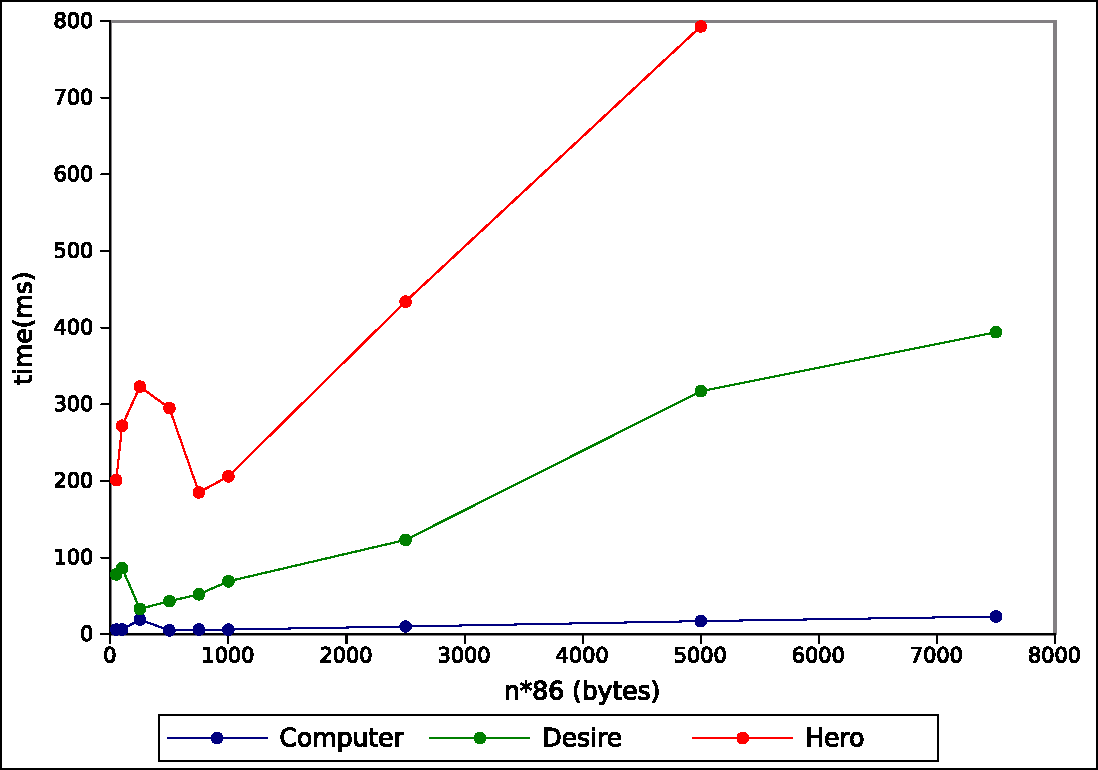
\includegraphics[scale=0.6]{graph_signandencrypt.pdf}
    \caption{Benchmark of how long it takes to sign and encrypt a folder}
    \label{fig:results:signencrypt}
\end{figure}
\begin{table}
  \centering
  \caption{Verify a folder of n*86 bytes. Time in ms}
  \begin{tabular}{ | l | l | l | l |}
    \hline
    \textbf{n*86 bytes} & \textbf{Computer} & \textbf{HTC Desire} & \textbf{HTC Hero} \\ \hline
    50      & <1    &3  & 10    \\ \hline
    100     & <1    &3  &  9    \\ \hline
    250     & <1    &3  & 11    \\ \hline   
    500     & <1    &4  & 11    \\ \hline
    750     & <1    &5  & 13    \\ \hline
    1000    &  1    &5  & 17    \\ \hline
    2500    &  3    &8  & 26    \\ \hline     
    5000    &  4    &14 & 41    \\ \hline 
    7500    &  6    &19 & N/A   \\ \hline 
  \end{tabular}
  \label{tbl:folder:verify}
\end{table}


We observe that the slowest part of folder operations are the initial key
generation and the serialization speed. Verification, encryption and signing is
satisfiable for all devices. We also note that the performance of signing and
encrypting, as well as verifying, seems to increase as the amount of
data gets larger. The serialization part behaves the exact opposite, where
performance drops when the amount of data gets larger. We also note that our
implementation struggles to handle large folders on the HTC Hero.

\section{Brute Force Local Keyring}
\label{sec:R:BFLK}

Results from running the \ac{BFDA} and \ac{CDA} against an encrypted keyring
are given in the following sections.

\subsection{\acl{BFDA}}

With \ac{BFDA}, we executed both a brute force and a dictionary attack to
estimate the amount of passwords we could test during the course of a second.

The results for both attacks are shown in Table \ref{tab:res_bf}. Results
are given for different numbers of \ac{PBKDF2} iterations in passwords per
second (PW/s). Figure \ref{fig:bfres} exhibits these numbers.

\begin{table}[!h]
    \centering
    \caption{Speed results of running \acs{BFDA}}
    \label{tab:res_bf}
    \begin{tabular}{| r | r | r |}
	\hline
	\ac{PBKDF2} iterations          &Brute force attack	    &Dictionary attack	\\
	\hline
	500                             &2240 PW/s                &2240 PW/s	\\
	\hline
	1000                            &1120 PW/s                &1110 PW/s	\\
	\hline
	2000                            &570 PW/s                 &560 PW/s	\\
	\hline
	4000                            &280 PW/s                 &280 PW/s	\\
	\hline
    8000                            &140 PW/s                 &140 PW/s \\
    \hline
    \end{tabular}
\end{table}


\begin{figure}[!h]
\centering
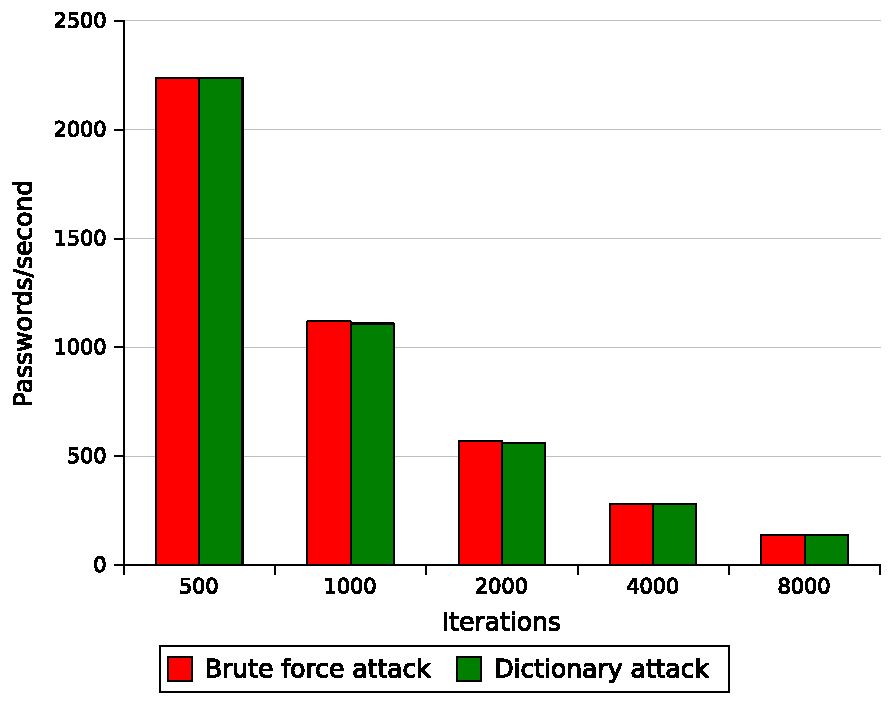
\includegraphics[scale=0.55]{graph_pbkdf2.pdf}
\caption{Results from running brute force and dictionary attacks against an encrypted keyring.}
\label{fig:bfres}
\end{figure}

Figure \ref{fig:bfres} indicates that by doubling the number of iterations in
PBKDF2, the efficiency of a brute force attack would decrease by half of
its value, as expected.

Using 1000 iterations in \ac{PBKDF2}, as recommended by \ac{NIST}
\cite{pbkdf_nist}, the brute force attack was able to reach a speed of around
1100 passwords per second. With this speed, it will take, in average, 39 hours
to crack a password with a length of 6 characters, consisting of small letters.

\subsection{\acl{CDA}}

When running \ac{CDA}, each node of the cluster achieved approximately the same
results as a single computer running a dictionary attack with \ac{BFDA}. We
found that there was a small difference where the local computer achieved about
50 passwords per second more, compared to an instance in the cluster.
The results may be due to the difference in \ac{CPU} power between the local
computer and a single cluster instance.

With 20 nodes in the cluster, we were able to test around 4600 passwords per
second, given \ac{PBKDF2} with 4000 iterations. Running \ac{CDA} in a cluster
of 200 nodes, should further reach a speed of 46 000 passwords per second.
Given a brute force attack with a speed of 46 000 password per second, it will
take about 289 283 years in average to brute force a password with the 10
character long alphanumeric password. Calculations are as follows.

\begin{align*}
\frac{62^{10} \text{ passwords}}{46000 \text{ passwords/second}} &= 18245638388442.18 \text{ seconds} \\
\frac{18245638388442.18}{60 * 60 * 24 * 365} &= 578565.40 \text{ years} \\
\frac{578565.40}{2} &= 289282.70 \text{ years in average}
\end{align*}

Given that the correct password is chosen completely random from the possible
set of passwords, the average time will represent the time used to brute force
half of the possible password space. The calculated time for brute forcing the
whole password space is therefore divided by two to get the average time.

At the time of writing, renting a single \emph{Amazon EC2 high-CPU extra large}
instance costs 0.68 USD per hour \footnote{From the price list at
\url{http://aws.amazon.com/ec2/pricing/}}. This unit price results in an hourly
cost of 13.6 USD and 136 USD for clusters of 20 and 200 instances respectively.

%**************************************%
\chapter{Discussion}
\label{ch:discussion}
%**************************************%

This chapter will discuss the proposed cryptographic scheme and its
implementation elaborated in Chapter \ref{ch:technical}, as well as
experimental findings in Chapter \ref{ch:results}. 

We will scrutinize the cryptographic scheme for its level of security and solid
features. Suggestions to support additional improvements are also considered.
Regarding the implementation, we will look at the choice of use case and
corresponding choice of key distribution. A suggestion to a simpler server-side
implementation is additionally given. We will finally discuss the performance
and security associated with the implementation.

\section{Cryptographic Scheme}

In this section, we will go through the cryptographic scheme proposed and
described in Section \ref{chap:CS}. Lastly, we analyse how the scheme does or
does not support various features and functionality.

\subsection{Security}

Even though we regard the proposed scheme as secure, some information will be
leaked both to the server, and potentially to an external attacker if a secure
channel for communication is not used.

The provider will be able to observe which folder is the root folder of a user.
This is because it will probably be the first folder a user creates, in
addition it will probably be the first folder a user accesses during each
session. The provider will also see which of kind of object is a
folder and which is a file, because a write enabler is sent alongside a folder.
The sequence of objects that a user requests will also leak some information
about the file and folder hierarchy. Lastly, the sharing of objects is possible
to determine based on who accesses a given storage index.

We do not consider any of this information to be dangerous for the server to
possess, but if an external attacker obtains the write enabler for a folder,
this might cause some problems in regards to availability.

\subsubsection{Confidentiality}

Confidentiality is provided by encrypting data locally with a random key before
it is stored in the cloud. This implies that confidentiality can only be
breached by weaknesses in the cryptographic primitives, side-channel attacks or
attacks on the client.  Security of the client is discussed in Section
\ref{sec:clientsecurity}. 

It is obvious that confidentiality weights heavily on the strength of the
utilized cryptographic primitives. The recommended primitives in Section
\ref{sec:cryptoprimitivechoice} are believed to ensure confidentiality.  It is
also possible to change the recommended cryptographic primitives with future or
existing algorithms.

The proposed cryptographic scheme has an additional weakness that can possibly
end with a breach of confidentiality. Namely, the procedure taken to derive the
write key of a folder. The write key is the result of hashing the private key
used to sign a folder. Given an attack that can derive the private key from the
corresponding public key, it will be easy for an attacker to retrieve the write
key of the folder. While the cryptographic primitives recommended should make
this infeasible to do at the time of writing, it might be possible in the
future.  The write key could instead be generated from a \ac{CSPRNG}, which is
the case for the read key of files.

\subsubsection{Integrity}

The cryptographic scheme provides integrity by adding a cryptographic hash
value into the encrypted parent folder of a object that is stored in the
cloud. The hash value from a file is derived from its content, while the hash
value from a folder is generated from its public key. To breach integrity, an
attacker must be able to change a cryptographic hash value stored inside a
folder. This implies that both reading and writing to a folder is achieved.

With this in mind, the integrity of the cryptographic scheme relies on the
confidentiality provided by the encrypted folders. In other words, the
integrity builds on the underlying cryptographic primitives as well as the
client security.

\subsubsection{Non-repudiation}

It is possible, in the proposed cryptographic scheme, to confirm that a user
with access to the correct capability has changed a folder, ie. uploaded or
unlinked a file to the folder. The scheme does not provide the
information necessary to confirm which user changed the folder or when it
happened. It is possible, however, to implement this functionality on top of
the proposed scheme to provide non-repudiation in the accounting layer.

\subsubsection{Authentication}

One could argue that the proposed scheme does not include authentication, but
at the same time one could argue that the possession of a capability
authenticates a user. If authentication is not implemented as an extra layer as
described in Section \ref{sec:accounting}, the server does not really
authenticate the user.  Granted the knowledge of the storage index does
indicate possession of the capability, but this index can theoretically be
stolen by using traffic analysis if the communication channel is not secured.
The possession of a capability does authentication in some way, but not the
user. Rather it authenticates the capability, and at the same time grants
authorization to the otherwise useless encrypted data.

\subsubsection{Access Control}

Access to a resource in the proposed scheme is given by capabilities.
Anyone can download any encrypted data from the server if they possess a
storage index, but that does not give access to the data. The possession of a
capability does however grant this access. 

The server will only need to handle write enablers in regard to access control.
Knowledge of the write enabler indicates knowledge of the write key which again
indicates possession of the whole capability. This means that access control in
this context is also given by the capability. The write enabler is vulnerable
to traffic analysis and other attacks that compromise availability if it is not
sent over a secure channel. An improvement of the scheme that could reduce the
risk of this, is to have the server actually verify that folders uploaded have
a correct signature. With that improvement, the write enabler is strictly not
necessary, but this will increase the requirements of the server.

\subsubsection{Availability}

The proposed scheme does not try to provide availability in regards to the
storage provider. The provider might chose to delete all data, or shut down the
server at any time. Tahoe-\ac{LAFS} has solved this by using erasure coding and
storing the data on different nodes. The result is that some nodes might be
taken down, but as long as a sufficient number is available, the data will also
be. This would also be possible with the proposed scheme, but is considered out
of scope for this thesis.

If a secure communication channel is not used, availability will be a problem
in regards to an external attacker. By using traffic analysis, write enablers
can be obtained, which means that data can also be overwritten. A \ac{MITM}
attack could use modification of message to either prevent a user from storing
data or to make the user store wrong data. These attacks do not compromise the
confidentiality of the data, and they will be discovered by the integrity check
failing. A possible attack, that is not detected by the integrity check, is the
replay attack. The attacker can record an update of a folder and replay that
message when the folder has further been updated causing possible loss of data.

\subsubsection{Sharing}

One of the major advantages of \ac{CSV} over many cloud storage systems, is the
possibility to share files and folders in a secure manner. If only the read
capability of a folder is shared, the user holding the write capability are
guaranteed to be the only one capable of making valid changes to the folder.

The server denies people with only the read capability to make changes to the
folder by the use of the write enabler. The write enabler serves the
purpose of proving to the server that one holds the correct write capability.
If someone with access to the file system on the server, e.g. a cloud
provider employee, decides to make changes on a folder, the integrity check
will warn the user of this.

\subsubsection{Supporting Multiple Cryptographic Primitives}

The main problem with selecting cryptographic primitives for our scheme, is
that one cannot be sure how long they will remain secure. A recommended
approach is to build systems that can easily change the cryptographic
primitives, in case of discoveries enabling an attacker to break a primitive
\cite{schneier}. The main problem with this approach is that if for instance
\ac{AES} is broken, and the cloud provider keeps backups of all user data on
their server, that information could be compromised with regard to the
provider.

A change of a cryptographic primitive in our scheme would lead to backward
compatibility being broken, i.e. one would be unable to obtain files or folders
stored before the change. This could be remedied by a meta block for each file
and folder, containing the utilized cryptographic primitives. In addition, the
capability would have to contain which cryptographic hash function that should
be used, to be able to deduce the storage index from the key.

\section{Implementation}
\label{sec:DIS:impl}

This section will discuss and deal with the different choices taken to fulfil
the implementation of the cryptographic scheme. We will start by discussing the
use case we chose to implement. Further on, we will analyse our choice of key
distribution scheme and look at alternative solutions. Lastly, we will discuss
the performance and security of the client implementation.

\subsection{Choice of Use Case}

There are mainly two types of user groups interested in a cloud storage
solution -- personal or enterprise. The proof of concept implementation is more
aimed against the personal use case, than the enterprise market.

In an enterprise, the use of a \ac{TTP} are often already in place, usually in
the form of an IT department. An additional fundamental difference, is that it
would usually be more defined who the users are supposed to share files with,
and what they should have access to. An organization might not approve of a
model where all users can forward read rights to other users.

\subsection{Key Distribution}

Our solution for key distribution is by no means revolutionary, it does require
two users to meet each other to exchange keys. However, the scheme only require
that users meet each other once, all sharing after that can be done with no
contact between the two parties. The use of barcodes for transferring keys on
smart phones also makes the process of actually handing over a key much easier.
In addition, the manual import option in the client grants every user the
possibility of using any other channel for transferring keys.


\subsection{Simplifying the Server}

The implemented proof of concept server generally performs quite well, and was
never identified as a bottleneck during the performance measurements. However,
by making the server-side contain less logic, \ac{CSV} could be used against
for instance the Amazon S3 service. This would more easily enable users that
are not comfortable with setting up a web server, to set up the whole system
from scratch. Another possibility is that the cloud provider could run the
server as \ac{IaaS}.

By redesigning the scheme to use a \emph{dumb file store}, the write enabler
functionality will be lost. However, a service like Amazon S3 do provide some
access control, and in the scenario of a \emph{friend net}, this could actually
be considered as a better solution. Luckily, the cryptographic architecture
presented in Section \ref{chap:CS}, are loosely coupled with the accounting
layer, so extending the proof of concept software to use a dumb file store
should not pose any great concerns.

\subsection{Performance}

The measurements performed on our client reveal that it has some performance
issues with regards to the speed of downloads and uploads. For files, a perfect
client would render the network or the memory card as the bottleneck, but our
measurements state that this is not the case. However, we find the
performance obtained by both the computer and the HTC Desire as satisfiable.
The HTC Hero struggles with certain operations, but is at the same time an
older device with limitations in both \ac{CPU} and memory capacity.

Because of the cryptographic operations, the download and upload speed for a
given file is decreased by around 50-80\% on all three devices. The results for
the individual operations performed on HTC Desire shown in Table
\ref{tbl:desire:pinpoint}, indicates that encryption and decryption are the
slowest elements in the process pipeline, and responsible for most of the
performance drop.

\paragraph{Limitations of Libraries} Another thing to note, is that the
implementations of the \texttt{InputStream} and \texttt{OutputStream} objects
in Java and the Apache HttpComponents seems to read and write the requested
number of bytes stream by stream. This implies that the implementation will
never reach the speed achieved by the slowest component in the pipeline.

\paragraph{Multiple CPU Cores} Branching the operations in the pipeline to
different threads should make it possible to gain better performance,
especially in an environment which spots multiple processor cores. Multiple
\ac{CPU} cores is standard on modern computers, and there is no reason to
suspect otherwise than that also smart phones will be equipped with this in the
nearest future. In addition, dedicated cryptographic coprocessors may
relieve the \ac{CPU} from additional work.

\paragraph{Folders} The performance of the folder operations in the
implementation is quite good, if we look at the cryptographic
functionality. We identify the slowest operation to be the generation of
new cryptographic keys. For a user of the Android client, this should not be a
problem, since the folder creation is done as an asynchronous task while the
user enters the name of the new folder. Another solution is to have the
application maintain a pool of keys before they are requested by the user. In
this way a key can almost always be ready for the user when needed.

The other cryptographic operations on folders completes quite quickly, but the
performance for serializing the folder contents is too low when folders contain
a large number of items. A folder with thousands of children is not
something we expect an ordinary user of the Android client to have, but if we
change the scenario to backing up an entire computer, the serialization part
might become a problem.

The slow serialization operation can partially be blamed on our own
implementation. The folder items are stored in a \texttt{HashMap}, which is
serialized to a string to make it ready for encryption. Ideally, this step is
not necessary, given that the folder contents exists in its correct form in
memory. This might not be possible due to reasons such as decreased performance
when manipulating the folder content. But we believe it is possible to create a
faster implementation of the currently utilized serialization algorithm.

\paragraph{Cache} Since opening folders is a relatively expensive procedure,
given that it has to be downloaded from the server, decrypted and verified, we
keep the currently opened folder and its parents in a stack. This can be seen
as a kind of cache, and could be extended to include all folders opened
in the active session.

\subsection{Client Security}
\label{sec:clientsecurity}

If a user physically looses her device, and the \ac{CSV} software is running,
anyone who finds the device can get access to the user's private files and
folders. This is because the client software will have to keep the root
capability from the keyring in memory, and will potentially have copies of the
files on the device. The same applies if the device is broken into, e.g.
through a vulnerability in the operating system.

\subsubsection{Downloaded Files}

An attacker who gains access to the device running \ac{CSV} will be able to
read downloaded files. It is possible to avoid writing downloaded files to the
persistent storage medium. This can be implemented using a temporary file
system that only persists in the memory of the client, e.g. \emph{ramfs}. This
is a file system for clients running Unix-like operating systems.  However,
utilizing this method will limit the possible size of the downloaded files to
the size of the available memory.

In case limited file size is not an acceptable solution, it is possible to use
a temporary file system that supports swapping, e.g. \emph{tmpfs}.  This will,
however, potentially keep parts of a large file on the persistent storage
medium, revealing information about a downloaded file. A practical feature
would be to store the encrypted files on the persistent storage medium, and
only put them in the temporary file system when needed.

\subsubsection{Disclosing the Root Capability}

The confidentiality of the root capability is held by an encrypted keyring that
is stored client-side. The keyring is encrypted with a key derived from a
password provided by the user. Unfortunately, using a password to encrypt the
keyring, makes the keyring a suitable target for brute force and dictionary
attacks. The vulnerability of the keyring against brute force and dictionary
attacks was questioned in Section \ref{sec:BFLK}.

\paragraph{Brute Forcing the Keyring} From the results in Section
\ref{sec:R:BFLK}, we noticed that the choice of iterations in \ac{PBKDF2} were
conclusive to the efficiency of a brute force attack against the encrypted
keyring. By doubling the number of iterations in \ac{PBKDF2}, the efficiency of
a brute force attack would decrease by a corresponding 50\%.

When following the recommendations for \ac{PBKDF2} and password constraints
given in Section \ref{sec:PBKD}, it is infeasible to perform a brute force
attack against the encrypted keyring. However, even though the keyring is
secured against a brute force attack, it is still vulnerable to dictionary
attacks due to the passwords being made by humans. To completely prevent such
attacks, one would have to make sure that the encrypted keyring is never
disclosed.

Our implemented attacks were not very effective against the keyring, but both
\ac{CDA} and \ac{BFDA} may be subject to improvement. An example to increase
efficiency would be to design the programs to run on \acp{GPU} rather than
\acp{CPU}. We are also not sure that the cryptographic primitives supplied by
Bouncy Castle are the fastest available. Considering findings by
\citet{rothwpa}, it is reasonable to believe that the keyring is more
vulnerable to brute force attacks than what our attacks imply. However, even
with the speed obtained by Roth, a brute force attack seems infeasible, while a
dictionary attack will always be possible and its success strongly dependant on
the chosen password.

\paragraph{Active Attacks}

While the encrypted key ring may resist some dictionary and brute force
attacks, other problems arise when facing an active attacker. If the attacker
is able to read the memory of the device, she can also read the root capability
if this is unlocked by the user.

A mechanism that decrease the risk of this happening, is to have the software
time out after a specified interval. At the timeout the software can overwrite
the sensitive information in memory.

Another scenario would involve the attacker installing a \emph{keylogger} on
the compromised client. This type of software can further detect the keyring
password when the user logs in to the application.

\chapter{Future Work}
The proposed cryptographic scheme has multiple features that can be added and
improved. In the following sections, we present what we see as the most
important ones.

\section{Key Distribution}
\label{sec:DI:keydist}

The challenge of key distribution in a user friendly way is hard. To
successfully authenticate a user and transfer a key, it is possible to choose
from the following methods:

\begin{itemize}
 \item Use a trusted third party
 \item Meet a user in person
 \item Use some sort of safe out of bound channel
\end{itemize}

Since one of the basic problems of this thesis is that the cloud provider is
not to be trusted, it is not desirable to use a trusted third party. This
implies that the only option left, is to verify another user in person,
although an out of band scheme like \ac{PGP} could be used.

In \ac{PGP}, users can publish that they have verified other users and to which
degree they trust them \cite{stallings}. Other users can use this information
to calculate the probability that a certain user is legit. The reason why this
scheme is not implemented, is that it is fairly complex for a standard user to
grasp. There are however nothing that stops a user that want to use the
\ac{PGP} scheme to transfer capabilities.

If the cryptographic scheme presented in Section \ref{chap:CS} should be used
in an organization, a \ac{PKI} is probably the best solution. In this setting,
the organization can itself be the trusted third party that enforces that all
certificates granted to users are correct. A user could then simply be prompted
by the name of the user she would like to share a file with, and the rest could
be handled by software logic and the trust of the \ac{PKI}.

\section{Deletion of Files}
\label{sec:deletion_of_files}

To support deletion of files, various alternatives has to be assessed.
Consider the following scenarios:

\begin{enumerate}
  \item A folder is shared between two users, and one of the users has
    linked in the files in other directories as well. What should happen if the
    other user deletes the files in the shared folder?

  \item A folder contains a folder which is a link to a folder ``higher''
    in the folder tree, and thus creating a loop. By deleting the folder,
    should all subdirectories be deleted as well, i.e. cascading delete?
\end{enumerate}

The choice of the alternatives presented shortly, are not taken by the proposed
cryptographic scheme, as it is merely a practical decision.

To remedy the problem of cascading deletion with loops, the system could
utilize an algorithm for finding \emph{strongly connected components} of a
graph, before actually deleting any files.

Two components are strongly connected if there exist a path from $A$ to $B$,
and from $B$ to $A$, as depicted in Figure \ref{fig:DSC:cycles} where a
directory is linked in at a higher level in the directory tree. The dashed line
represents the actual path in the graph. If the folder $X$ is requested to be
deleted, the $A$ and $Y$ directories are also removed. This behaviour may not be
expected nor desired by the user.

\begin{figure}[h!]
    \centering
    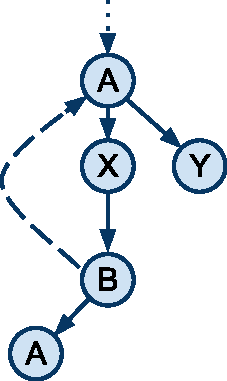
\includegraphics[scale=0.6]{CyclesintheDAG.pdf}
    \caption{Theoretical cycle in the directory graph}
    \label{fig:DSC:cycles}
\end{figure}

\emph{Tarjan's Algorithm} \cite{tarjan} is an example of algorithm that can be
implemented to do this kind of check, and is basically a depth first search,
with a stack containing visited nodes.

\paragraph{Creator} The accounting layer on the server could store the
username of the creator of the file along with each storage index, and use this
to decide who should be granted access to delete files.

\paragraph{Write Enabler} Similarly, the server could grant removal rights to
whoever provides the write enabler, in the same manner as when updating
folders. This requires that \emph{delete enablers} is produced for immutable
files.

\paragraph{Link Count} The files could include a link count in its meta data,
which is updated whenever a user links or unlinks it from a folder. When the
link count reaches zero, the user notifies the server to delete it. This would
have to be combined with the use of delete enablers for files.

\section{Verification of Files}

The verification scheme for immutable files is suboptimal in every way a user
wants to use an ordinary file. The problem is that the user will have to
download the entire file, before she can verify that the file is what it is
supposed to be. If it turns out that the file does not pass this check, and the
error was in the very first byte, the user has wasted time and bandwidth
downloading a lot of useless data. The same scenario applies if the user only
wants to look at a small part of a file, e.g. the middle section of a movie, or
to utilize the file while it is still downloading.

A possible solution to support this kind of verification, would be to build a
\emph{hash tree} of the whole file, as shown in Figure \ref{fig:hashtree}. With
a hash tree, smaller parts of the file can be verified, and errors can be
detected earlier. The hash tree could be stored encrypted on the server
together with the encrypted file, and the capability could hold the root hash
of the tree. The downside to this approach, is that performance would be
affected due to the substantial amount of hash operations required to compute
the hash tree. This idea of a hash tree is implemented in Tahoe-\ac{LAFS}
\cite{tahoe}.

\begin{figure}[!h]
\centering
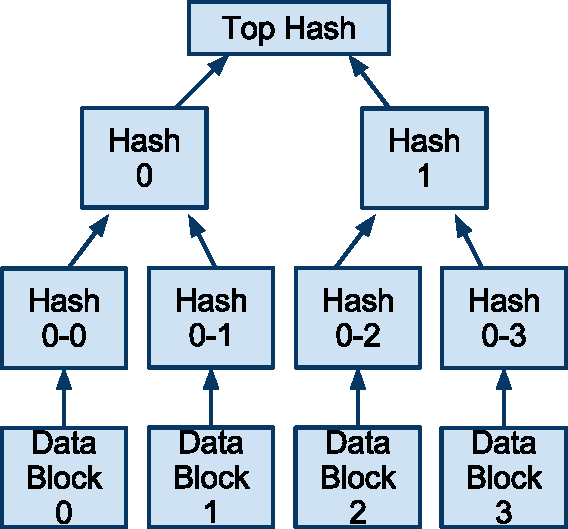
\includegraphics[scale=0.55]{hash-tree.pdf}
\caption{Hash tree of a file}
\label{fig:hashtree}
\end{figure}

\section{Version Control System}

Some of the currently available cloud storage systems, as Wuala and Dropbox
mentioned in Section \ref{sec:existing}, support a kind of \emph{version
control} of the files stored. This means that the data lost during a
modification of a file are saved alongside the current file, so that the user
has enough information to restore the file to a previous state.  In practice,
this often mean to store multiple versions of the same file, or the difference
between two versions. This could be implemented in \ac{CSV} by one of the
following methods.

\paragraph{Extension to Folders} By adding a list of subsequent files to the
directory structure exemplified in Section \ref{sec:cli:impl:det}, we can link
previous versions of a file in the serialization form:

\begin{quote}
    \centering
    \textbf{alias;capability;capability;capability}
\end{quote}

To make this feasible and user friendly, a time stamp would have to be added to
the capability. This would increase the size of the folder.

\paragraph{Type of Mutable File} A new form of mutable file could be
implemented in practically the same form as a directory, containing timestamps
instead of aliases, and pointing to corresponding storage indexes. With this
procedure, it should be easy to configure for the user which files and folders
that should be under version control.

\section{Deduplication}

The term \emph{data deduplication} implies not having to store redundant data.
By implementing a deduplication scheme, multiple advantages can arise in the
sense of a storage system. For the service provider, this could mean cost
savings in the form of not having to store the same file twice, but still claim
money from users for the given storage. For the users of the service, this
could mean better network utilization, as uploading a big file that already
exist on the server would take no time at all.

However, there are practical disadvantages and great privacy concerns related
to deduplication, in addition to some solutions that address these issues.  The
scheme does not support deduplication. This is because all encryption keys are
randomly selected, neither the server or the client is able to detect whether a
file already exists in the system.

\paragraph{Practical Disadvantages} Deduplication relies on the use of hash
functions to check whether a file or a block of data exist on the storage node.
In general, as long as you hash something larger than the length of the digest,
there exists collisions, and hence data corruption.

Further on, the additional hash operations and queries to the server pose
extra computational overhead, which increase if the deduplication is on block
level.

\paragraph{Privacy} If deduplication is used on file-basis globally -- i.e.
for all users -- there exist a privacy risk. The provider will be able to prove
that a certain file exists on the system, and has the ability to figure out
which user has saved this file thus effectively compromising the
confidentiality of that file. If the deduplication scheme works in a manner in
which the file is not uploaded if it already exists on the server any user is
able to prove that a file is already stored.

\paragraph{Customizable Deduplication} Tahoe-\ac{LAFS} tries to provide a
solution that has all the advantages and none of the issues related to
deduplication, by \emph{convergent encryption with an added secret}
\cite{tahoe}.

Convergent encryption implies using the hash of the plaintext as the key to the
symmetric encryption algorithm, i.e. the same plaintext will always yield the
same ciphertext, making it easy to implement deduplication.

Tahoe-\ac{LAFS} adds a per-client secret to the hashing procedure, as
depicted in Figure \ref{fig:tahoe:dedup}, before using the result as a key to
encrypt the file. This enables per-client deduplication, or per-group
deduplication if the user shares the secret with other users. Since the storage
index is based on the encryption key, and the plaintext will always lead to the
same encryption key, the client can check for file existence on the server and
prevent duplication.

\begin{figure}[!h]
    \centering
    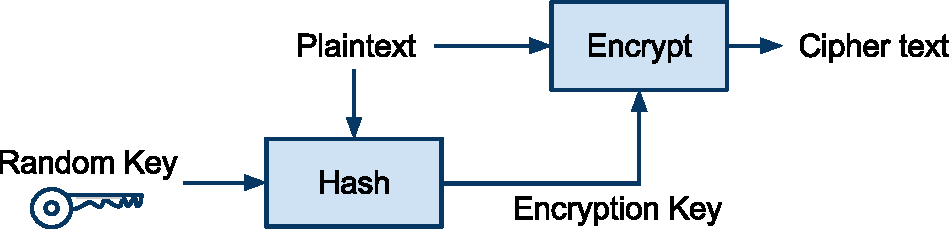
\includegraphics[scale=0.55]{TahoeDeduplication.pdf}
    \caption{Tahoe-LAFS deduplication scheme}
    \label{fig:tahoe:dedup}
\end{figure}

\section{Implementation}
\label{sec:DIS:impl}

This section will discuss and deal with the different choices taken to fulfil
the implementation of the cryptographic scheme. We will start by discussing the
use case we chose to implement. Further on, we will analyse our choice of key
distribution scheme and look at alternative solutions. Lastly, we will discuss
the performance and security of the client implementation.

\subsection{Choice of Use Case}

There are mainly two types of user groups interested in a cloud storage
solution -- personal or enterprise. The proof of concept implementation is more
aimed against the personal use case, than the enterprise market.

In an enterprise, the use of a \ac{TTP} are often already in place, usually in
the form of an IT department. An additional fundamental difference, is that it
would usually be more defined who the users are supposed to share files with,
and what they should have access to. An organization might not approve of a
model where all users can forward read rights to other users.

\subsection{Key Distribution}

Our solution for key distribution is by no means revolutionary, it does require
two users to meet each other to exchange keys. However, the scheme only require
that users meet each other once, all sharing after that can be done with no
contact between the two parties. The use of barcodes for transferring keys on
smart phones also makes the process of actually handing over a key much easier.
In addition, the manual import option in the client grants every user the
possibility of using any other channel for transferring keys.


\subsection{Simplifying the Server}

The implemented proof of concept server generally performs well, and was never
identified as a bottleneck during the performance measurements. However, by
making the server-side contain less logic, \ac{CSV} could be used against for
instance the Amazon S3 service. This would more easily enable users that are
not comfortable with setting up a web server, to set up the whole system from
scratch. Another possibility is that the cloud provider could run the server as
\ac{IaaS}.

By redesigning the scheme to use a \emph{dumb file store}, the write enabler
functionality will be lost. However, a service like Amazon S3 do provide some
access control, and in the scenario of a \emph{friend net}, this could actually
be considered as a better solution. Luckily, the cryptographic architecture
presented in Section \ref{chap:CS}, are loosely coupled with the accounting
layer, so extending the proof of concept software to use a dumb file store
should not pose any great concerns.

\subsection{Performance}

The measurements performed on our client reveal that it has some performance
issues with regards to the speed of downloads and uploads. For files, a perfect
client would render the network or the memory card as the bottleneck, but our
measurements state that this is not the case. However, we find the
performance obtained by both the computer and the HTC Desire as satisfiable.
The HTC Hero struggles with certain operations, but is at the same time an
older device with limitations in both \ac{CPU} and memory capacity.

Because of the cryptographic operations, the download and upload speed for a
given file is decreased by around 50-80\% on all three devices. The results for
the individual operations performed on HTC Desire shown in Table
\ref{tbl:desire:pinpoint}, indicates that encryption and decryption are the
slowest elements in the process pipeline, and responsible for most of the
performance drop.

\paragraph{Limitations of Libraries} Another thing to note, is that the
implementations of the \texttt{InputStream} and \texttt{OutputStream} objects
in Java and the Apache HttpComponents seems to read and write the requested
number of bytes stream by stream. This implies that the implementation will
never reach the speed achieved by the slowest component in the pipeline.

\paragraph{Multiple CPU Cores} Branching the operations in the pipeline to
different threads should make it possible to gain better performance,
especially in an environment which spots multiple processor cores. Multiple
\ac{CPU} cores is standard on modern computers, and there is no reason to
suspect otherwise than that also smart phones will be equipped with this in the
nearest future. In addition, dedicated cryptographic coprocessors may
relieve the \ac{CPU} from additional work.

\paragraph{Folders} The performance of the folder operations in the
implementation is good, if we look at the cryptographic functionality. We
identify the slowest operation to be the generation of new cryptographic keys.
For a user of the Android client, this should not be a problem, since the
folder creation is done as an asynchronous task while the user enters the name
of the new folder. Another solution is to have the application maintain a pool
of keys before they are requested by the user. In this way a key can almost
always be ready for the user when needed.

The other cryptographic operations on folders completes quickly, but the
performance for serializing the folder contents is too low when folders contain
a large number of items. A folder with thousands of children is not something
we expect an ordinary user of the Android client to have, but if we change the
scenario to backing up an entire computer, the serialization part might become
a problem.

The slow serialization operation can partially be blamed on our own
implementation. The folder items are stored in a \texttt{HashMap}, which is
serialized to a string to make it ready for encryption. Ideally, this step is
not necessary, given that the folder contents exists in its correct form in
memory. This might not be possible due to reasons such as decreased performance
when manipulating the folder content. But we believe it is possible to create a
faster implementation of the currently utilized serialization algorithm.

\paragraph{Cache} Since opening folders is a relatively expensive procedure,
given that it has to be downloaded from the server, decrypted and verified, we
keep the currently opened folder and its parents in a stack. This can be seen
as a kind of cache, and could be extended to include all folders opened
in the active session.

\subsection{Client Security}
\label{sec:clientsecurity}

If a user physically looses her device, and the \ac{CSV} software is running,
anyone who finds the device can get access to the user's private files and
folders. This is because the client software will have to keep the root
capability from the keyring in memory, and will potentially have copies of the
files on the device. The same applies if the device is broken into, e.g.
through a vulnerability in the operating system.

\subsubsection{Downloaded Files}

An attacker who gains access to the device running \ac{CSV} will be able to
read downloaded files. It is possible to avoid writing downloaded files to the
persistent storage medium. This can be implemented using a temporary file
system that only persists in the memory of the client, e.g. \emph{ramfs}. This
is a file system for clients running Unix-like operating systems.  However,
utilizing this method will limit the possible size of the downloaded files to
the size of the available memory.

In case limited file size is not an acceptable solution, it is possible to use
a temporary file system that supports swapping, e.g. \emph{tmpfs}.  This will,
however, potentially keep parts of a large file on the persistent storage
medium, revealing information about a downloaded file. A practical feature
would be to store the encrypted files on the persistent storage medium, and
only put them in the temporary file system when needed.

\subsubsection{Disclosing the Root Capability}

The confidentiality of the root capability is held by an encrypted keyring that
is stored client-side. The keyring is encrypted with a key derived from a
password provided by the user. Unfortunately, using a password to encrypt the
keyring, makes the keyring a suitable target for brute force and dictionary
attacks. The vulnerability of the keyring against brute force and dictionary
attacks was questioned in Section \ref{sec:BFLK}.

\paragraph{Brute Forcing the Keyring} From the results in Section
\ref{sec:R:BFLK}, we noticed that the choice of iterations in \ac{PBKDF2} were
conclusive to the efficiency of a brute force attack against the encrypted
keyring. By doubling the number of iterations in \ac{PBKDF2}, the efficiency of
a brute force attack would decrease by a corresponding 50\%.

When following the recommendations for \ac{PBKDF2} and password constraints
given in Section \ref{sec:PBKD}, it is infeasible to perform a brute force
attack against the encrypted keyring. However, even though the keyring is
secured against a brute force attack, it is still vulnerable to dictionary
attacks due to the passwords being made by humans. To completely prevent such
attacks, one would have to make sure that the encrypted keyring is never
disclosed.

Our implemented attacks were not effective against the keyring, but both
\ac{CDA} and \ac{BFDA} may be subject to improvement. An example to increase
efficiency would be to design the programs to run on \acp{GPU} rather than
\acp{CPU}. We are also not sure that the cryptographic primitives supplied by
Bouncy Castle are the fastest available. Considering findings by
\citet{rothwpa}, it is reasonable to believe that the keyring is more
vulnerable to brute force attacks than what our attacks imply. However, even
with the speed obtained by Roth, a brute force attack seems infeasible, while a
dictionary attack will always be possible and its success strongly dependant on
the chosen password.

\paragraph{Active Attacks}

While the encrypted key ring may resist some dictionary and brute force
attacks, other problems arise when facing an active attacker. If the attacker
is able to read the memory of the device, she can also read the root capability
if this is unlocked by the user.

A mechanism that decrease the risk of this happening, is to have the software
time out after a specified interval. At the timeout the software can overwrite
the sensitive information in memory.

Another scenario would involve the attacker installing a \emph{keylogger} on
the compromised client. This type of software can further detect the keyring
password when the user logs in to the application.

%**************************************%
\chapter{Conclusion}
\label{ch:conclusion}
%**************************************%

The main purpose of this thesis was to create and implement a solution to a
secure cloud storage service. The scheme was to provide what we defined in
Chapter \ref{ch:intro} as a secure storage system.

Key elements of the proposed cryptographic scheme is based on the secure and
relatively scrutinized file system Tahoe-\ac{LAFS}. With this in mind, and the
use of cryptographic primitives recommended in Section
\ref{sec:cryptoprimitivechoice}, the proposed cryptographic architecture is
believed to offer a secure storage system.

In Section \ref{sec:R:BFLK}, attempts were made to attack the locally encrypted
keyring. The findings did not reveal any obvious weaknesses, but results from
another researcher indicates that dictionary attacks are feasible. However, to
acquire the keyring, an active attack on the client device is required. In
addition, measuring performance on constrained devices proved that the
trade-off between the levels of usability and security did not undermine the
desired strength of the underlying cryptographic primitives. For older devices,
the transfer speeds might not be satisfiable.

When developing a secure file system, one of the greatest challenges
turned out to be the choice and implementation of cryptographic primitives.
Good references and external recommendations can help, but only to a certain
degree. Key distribution is also a general problem that will always be hard to
accomplish, if a trusted third party is not to be included. Yet another
challenge experienced, is that all additional features desired for a secure
cloud file system are hard to implement without compromising security.
Deduplication is an example of this.

We have shown that it is possible to create and implement a fundamental
cryptographic scheme for a secure cloud storage system, supporting sharing.
The scheme does not require a specific key distribution method, but provides
the choice of implementing any desired solution on top. We have also
implemented an open source, proof of concept server and client for Android
devices, that have further been measured in performance and evaluated in
security. The client support easy exchange of keys by using barcodes.

While our scheme solves some of the basic challenges of security within cloud
storage, there are several features that could improve the scheme. The most
important being a better approach to verifying files, to e.g. allow streaming,
and the possibility of deleting files. For our implementation it would be
interesting to see a modified version which could work directly with
an existing \emph{dumb} cloud storage solution, such as Amazon S3.

%**************************************%
\bibliographystyle{unsrtnat} % BibTeX bibliography lives in external file
\bibliography{references}
%**************************************%

%**************************************%
\appendix
\appendixpage
\addappheadtotoc
%**************************************%
%**************************************%
\chapter{\acs{BFDA} and \acs{CDA} Implementations}
\label{ap:other}
%**************************************%

This chapter contains details about the implementations of \ac{BFDA} and
\ac{CDA}.

\section{Brute Force and Dictionary Attack}

\emph{\ac{BFDA}} includes a plain brute force attack and a dictionary attack against
a user's encrypted keyring. Details about the implementation follows.

\subsection{Implementation Details}

\ac{BFDA} is written in Java and utilize the \texttt{javax.crypto} library with
Bouncy Castle version 1.34 as JCE provider to decrypt the encrypted keyring.
The Bouncy Castle JCE provider seems to be necessary as Android uses it by
default to encrypt using AES. For \ac{PBKDF2} \ac{BFDA} utilizes a free
Java library\footnote{\url{http://rtner.de/software/PBKDF2.html}}.

The program is divided into two functions, named \texttt{bruteForceAttack} and
\texttt{dictionaryAttack}, that correspondingly executes a brute force and
dictionary attack. The \texttt{bruteForceAttack} function is shown in Listing
\ref{lst:bffunc}.

\clearpage
\lstinputlisting[language=java, label=lst:bffunc, caption=bruteForceAttack
function]{listings/bruteForceAttack.java}

\texttt{bruteForceAttack} starts a number of \texttt{BruteForceThread} threads.
The function continues after all \texttt{BruteForceThreads} are initialized and
ready to start their task. It then enters a while-loop, which executes a
\texttt{pushWord} function for each iteration.

The task of \texttt{pushWord} is to simply create and push all possible words
of a given length onto a stack of words. The length of the words to push are
given by its integer argument. The whole attack is based on letting the main
thread create and push words onto a stack, while the \texttt{BruteForceThreads}
are pulling words from it. When a word is pulled, it is subject to
\emph{PBKDF2}, where the result is used to decrypt the ciphertext. If
decryption results is a given plaintext, the password has been recovered.

The \texttt{dictionaryAttack} function is shown in Listing \ref{lst:dafunc}.

\lstinputlisting[language=java, label=lst:dafunc, caption=dictionaryAttack
function]{listings/dictionaryAttack.java}

\texttt{dictionaryAttack} reads an input dictionary file into a
\texttt{BufferedReader}. It then starts a given number of
\texttt{DictionaryThreads}. The \texttt{DictionaryThreads} will read from the
\texttt{BufferedReader} in a synchronized way. When a word is read from a
\texttt{DictionaryThread} it will be subject to \ac{PBKDF2}, where the result
is used to decrypt the ciphertext. If decryption results in a recognizable
plaintext, the password has been recovered.

\section{Cluster Dictionary Attack}

\ac{CDA} is written in Java, and is built around the same procedure as the
dictionary attack in \ac{BFDA}. However, the difference lays in the cooperation
of multiple computers. To enable a cluster of computers to cooperate, we used
the following environment.

\subsection{Environment}

The environment is based upon a software framework from Apache called
\emph{Hadoop}. The main functionality of Hadoop is described below.

\subsubsection{Apache Hadoop}

Apache Hadoop makes it possible for multiple machines to cooperate
and run computational work together. Hadoop also provides a distributed file system
\ac{HDFS}, that can store data across multiple cooperating machines \cite{hadoop}. The
computational work in Hadoop is organized and distributed using \emph{MapReduce}.

\paragraph{MapReduce} MapReduce is a programming paradigm introduced by Google.
It is designed to process and generate large sets of data using a cluster of
machines \cite{mapred}.

In MapReduce, a large set of input data is divided into multiple key-value
pairs. The key-value pairs are further distributed to multiple MapReduce tasks
running on multiple machines.

A MapReduce task is divided into a \emph{mapper} and a \emph{reducer}. The task
of a mapper is to perform an operation on a key-value pair and return a
key-value pair as a result to the reducer. The reducer collects pairs
from multiple mappers and combine the results into one or more output files.

\subsection{Implementation Details}

The \ac{CDA} attack is implemented as a MapReduce problem, with a large
dictionary file as the data input set. The dictionary is split into separate
key-value pairs, where each value is a single line in the dictionary and the
key corresponds to the number of that line.

The key-value pairs are handled by a map function implemented in
\texttt{CDAMapper}. The
map function has the responsibility of checking every word on a single
dictionary line. Each line in the dictionary should contain a certain amount of
words. This is to enable the map function to run multiple threads at the same
time, where each thread checks one or more words. With multiple threads, the
attack is able to utilize more \ac{CPU} power for each running machine in the
cluster. A detailed view of the map function, is given in Listing
\ref{lst:mapfunc}.

\lstinputlisting[language=java, label=lst:mapfunc, caption=Mapper function in
CDAMapper]{listings/mapper.java}

When receiving a key-value pair, the map function first splits the input line
into an array of words. It then creates a given number of
\texttt{DictionaryThread}s and serves each a subarray of words from the
array. Each \texttt{DictionaryThread} will check all of its incoming words
similar to the \texttt{DictionaryThread} in \ac{BFDA}. If the correct password is
found, the password will be written to the \texttt{sysout} folder.

A class named \texttt{Processor} initializes the \ac{CDA} attack by configuring
the mapper and reducer tasks. The number of mappers is set equal to the number
of nodes used in the cluster. This is to ensure that each machine only runs one
mapper at a time. The number of reducers are set to zero, because their
behaviour in MapReduce are not needed.

The for-loop at Line 10 in Listing \ref{lst:mapfunc} requires the number of
words per line, in the dictionary, to be equal to a multiple of the number of
threads in use. It is recommended that the input dictionary follows this
requirement. In this occasion, we have created a Bash script, named
\texttt{dictmaker.sh}, that changes a regular dictionary into an $N$
words-per-line dictionary. The script can be found on the attached disc.

%**************************************%
\chapter{Attachments}
\label{ap:attachments}
%**************************************%

This thesis comes with two available attachments -- one digitally uploaded to
the DAIM system\footnote{\url{http://daim.idi.ntnu.no/}}, and one physical disc.

\section{Electronic Attachment}

The electronic attachment, uploaded to DAIM, consists of the following files
and directories:

\begin{description}
  \item[Application] All files and source code of the proof of concept system,
    i.e. the background library, server and client. A patch file containing
    security fixes, is also included.
  \item[Other] Scripts and raw data from the experiments.
\end{description}

\section{Attached Disc}
The attached disc contains all contents also provided in the electronic
attachment, as well as a video demonstrating the Android client.

\end{document}
